\documentclass[a4paper, 12pt]{report}
\usepackage[top=3cm,left=1.5cm,right=1.5cm,bottom=1.5cm]{geometry}
\geometry{a4paper,top=30mm,bottom=20mm,left=15mm,right=15mm}
\usepackage[portuguese]{babel}
\usepackage[utf8]{inputenc}
\usepackage{cite}
\linespread{1.5}
\usepackage{verbatim}
\usepackage[hyperindex=true,colorlinks=true,linkcolor=blue,filecolor=blue,urlcolor=blue,bookmarks=false,hypertexnames=false]{hyperref}
\usepackage{amsmath,amsthm, amssymb,physics}
\usepackage{graphicx}
\usepackage{bbold}
\usepackage{stackrel}
\usepackage{float}
\usepackage{xcolor}

\usepackage{tikz}
\usetikzlibrary{positioning,fit,backgrounds}
\usepackage{graphicx}
% \newcommand{\com}[1]{}

\begin{document}

\begin{titlepage}
\begin{center}
\textbf{Universidade Estadual Paulista \textquotedblleft{Júlio de Mesquita Filho}\textquotedblright}\\
\textbf{Departamento de Ciências da Computação}\\
\vspace{2cm}
\textbf{Projeto de Pesquisa de Pós-doutorado}\\
\vspace{2cm}
\textbf{\textit{{\Large Título Pendente}}}\\
\vspace{2cm}
\textbf{Candidato à Bolsa:} Dr. Maicon carlone da Silva\\
\textbf{Supervisor:} Prof. Dr. ---%João Paulo Papa\\
\vspace{2cm}
\end{center}
\textbf{Resumo:}
O presente projeto apresenta uma metodologia nova para o estudo de imagens de Ressonância Magnética (MRI), sendo especialmente desenvolvida e instrumentalizada para os desafios do treino e uso de Redes Neurais Convolucionais (CNN) e sua respectiva implementação na computação quântica. É proposta a utilização de transposições espaciais específicas para as condições de simetria do problema, reduzindo a dimensionalidade do problema sem destruir ou negligenciar aspectos relevantes da informação. A presente abordagem foi desenvolvida com o propósito de buscar, avaliar e classificar anomalias elusivas, pouco evidentes ou completamente negligenciadas. Sendo assim, pode-se pressupor que a exploração da geometria oculta do problema, assim como das sutilezas morfológicas, podem se tornar indicativos proeminentes da existência de zonas ou corpúsculos anômalos.

\end{titlepage}

\begin{titlepage}
\begin{center}
\textbf{Universidade Estadual Paulista \textquotedblleft{Júlio de Mesquita Filho}\textquotedblright}\\
\textbf{Departamento de Ciências da Computação}\\
\vspace{2cm}
\textbf{Post-doctoral research project}\\
\vspace{2cm}
\textbf{\textit{{\Large Título Pendente }}}\\
\vspace{2cm}
\textbf{Candidate to the post-doctoral fellowship:} Dr. Maicon carlone da Silva\\
\textbf{Research Leader:} Prof. Dr. ---%João Paulo Papa\\
\vspace{2cm}
\end{center}
\textbf{Abstract:}
This project introduces a novel methodology for the analysis of Magnetic Resonance Imaging (MRI) data, specifically tailored for the training and application of Convolutional Neural Networks (CNNs) and their subsequent implementation in quantum computing. We propose the utilization of spatial transpositions, informed by the inherent symmetries of the problem, to achieve dimensionality reduction without compromising the integrity of salient informational aspects. This approach is designed to identify, evaluate, and classify elusive anomalies that are either subtle, non-evident, or conventionally overlooked. It is our hypothesis that by exploring the underlying geometry of the problem, subtle morphological features can be transformed into prominent indicators of anomalous regions or corpuscles.
\end{titlepage}

\hrule $\frac{}{}$\\
\begin{LARGE}
\textbf{1. Introdução}
\end{LARGE}
\\ \hrule $\frac{}{}$\par

O desenvolvimento acadêmico atual é contemporâneo ao nascimento e estabelecimento dos modelos de inteligência artificial (AI) como ferramentas indispensáveis para uma nova era das descobertas científicas \cite{KohArtificial2022,ZhangMachine2023,ZhangNovel2023,LiPerformance2019Nov,LiuEvolving2020Jan}. Este projeto é consoante com esta expectativa, aqui tais modelos serão empregados no estudo e identificação de tênues anomalias, captáveis em imagens, com o intuito de confecção de ferramentas de uso prático e aplicado em meio clínico e hospitalar.

Ao contrário do que é geralmente visto na literatura, não será objetivada a aplicação em si de imagens de secção de Ressonância Magnética (MRI) {\lq\lq}cruas{\rq\rq} no treinamento de modelos, tão pouco serão utilizadas técnicas comuns na redução da dimensionalidade do problema, tais como \textit{Principal Component Analysis} (PCA) \cite{JolliffePrincipal2016Apr}, \textit{Stochastic Neighbor Embedding} de Geoffrey Hinton (T-SNE) \cite{VanderMaaten2008} ou mais específicas para tratamento de imagens de MRI \cite{Plis2014}, mas sim uma elaboração única, que concilia a estrutura dimensional ao observável alvejado, ampliando as capacidades intrínsecas de detecção, obtidas pelo treinamento de modelos de AI.

Para isso, será definida uma metodologia de redução de dimensionalidade especialmente elaborada para a detecção e classificação de anormalidades elusivas em imagens, com o foco no estudo de MRI. O que proporcionará um novo conjunto de bioindicadores e mascaras \cite{Iqbal2018,Kumar2023, Liu2014}, que poderão e, seguramente, serão utilizados tanto como artifícios para treinamento, quanto para compreensão direta de análises laboratoriais.

Por intermédio da estruturação de um espaço de operações vetoriais, anomalias pouco aparentes, elusivas, ou até mesmo, não detectáveis, poderão ser evidenciadas devido ao seu impacto sobre a estrutura morfológica geral do objeto de estudo. Neste projeto, os resultados de transposições espaciais adversas serão denominados como construtos virtuais\footnote{O termo construto entoa um objeto passivo de classificação topológica, obstante, mas não desassociado de espaço Real.}. Ou seja, entidades que contemplam representações das componentes morfológicas fora do espaço real, onde características associadas a anomalias e patologias tornar-se-ão mais pronunciadas.

Diferente das técnicas usuais de propósito geral, a abordagem proposta parte das componentes simétricas observacionais presentes na estrutura cerebral. Em súmula, dois conjuntos de resultados serão obtidos. Um deles versa sobre a formulação de identidades ou \textit{brainprints}, diretamente correlacionados com estruturas ordinárias e patológicas. Enquanto o outro, propícia à identificação de operadores, que poderão ser obtidos do treinamento de modelos, e atuarão no lugar de máscaras tradicionais. Desse modo, serão obtidas identidades e operadores patológicos, cuja presença ou aplicação sobre o estado permitirá classificação e detecção de anomalias, sejam elas catalogadas ou não. 

Em conformidade com a expectativa da literatura \cite{Zitu2024Dec,Hays2024Dec,Binzagr2024Apr}, será provida uma metodologia que propicie a reconstrução dos resultados obtidos para o espaço Real, garantindo interpretação direta e não correlacionada ao formalismo empregado, assim como um mapeamento para uma representação com coesão direta à estrutura cerebral. Essa abordagem gerará resultados condizentes, ideais para utilização de técnicas de transferência de conhecimento para treinamento de Redes Neurais \cite{Hussain2024,Mane2024} ou reinserções.

$\frac{}{}$\\
\begin{Large}
	\textbf{1.1 Motivação}
\end{Large}
$\frac{}{}$\\

Em materiais, tanto em experimentos quanto em simulações de ESR, os momentos magnéticos podem ser perturbados pelo impacto do modo vibracional da rede na vizinhança eletrônica \cite{Carlone2022,Souza2020,Stankiewicz2023,Kim2014, Lesseux2017, Calvo1971}. De modo sucinto, o efeito ocorre por uma sequência curiosa de casualidades, sendo eles:

A variação do modo vibracional perturba o campo cristalino dos elementos que constituem a vizinhança eletrônica da sonda, sendo essa a responsável pela quebra da degenerescência e abertura dos níveis Zeeman. Com isso, consequentemente, uma perturbação é causada nos campos de ressonância aos quais a sonda está submetida, o que causa uma pequena variação em relação ao que seria esperado nas características obtidas no experimento de ESR, em especial, na forma da largura de linha.

Dito isso, mesmo que esse efeito tenha sido muito bem caracterizado para ESR, o mesmo deve ser esperado em retratações de MRI, se estabelecido um paralelo para a perturbação dos níveis de energia local, que afetam o momento magnético e por consequência suas componentes, culminando na alteração sútil das medidas de relaxação \cite{Carlone2022, Lesseux2017}. Contudo, é importante salientar que o descrito efeito é discrepante da maioria das discussões sobre modos na literatura \cite{Mariappan2010, Xu2007, Hamhaber2010, Xydeas2005}, visto sua correlação entre os modos e o tecido (\textit{Magnetic Resonance Elastography} - MRE), e não entre a perturbação local imposta pela possível interação entre momentos perturbados pelos modos. Em outras palavras a variação da resposta de ressonância pela mudança natural do modo vibracional pode, em tese, constituir um elemento observacional indireto já presente nas imagens de MRI, não dependente de inserção de aparato instrumental adicional.

Efetivamente, medidas espectrográficas tomadas sobre amostras reais, inferem sobre o comportamento médio dos momentos, pois cada momento presencia leves variações em sua vizinhança local \cite{Abragam1961}. Curiosamente, mesmo dentro de uma delimitação bio-estrutural, existem pequenas variações na resposta de ressonância captada, o que pode estar correlacionado a variações locais de temperatura impostas pela atividade biológica, erros esperados, entre outras causas prováveis \cite{Lauterbur1973}. Com a discussão passada em mente, e sabendo sobre o impacto do modo vibracional nos momentos localizados, a seguinte suposição pode ser feita:

Estruturas anômalas {\lq\lq}imersas{\rq\rq} em estruturas ordinárias, podem causar uma disruptura da homogeneidade da intensidade dos momentos locais vizinhos, o que, por consequência, afeta a resposta de ressonância captada. Pode-se supor que essas estruturas anômalas constituam-se de pequenas densidades corpusculares que estão {\lq\lq}solutas{\rq\rq} em uma estrutura biológica conhecida, de modo que, nem ao menos são grandes o suficiente para serem reconhecidas e caracterizadas em uma imagem, ainda assim, seu diferente modo vibracional deve causar uma perturbação na vizinhança local, perturbação essa, que poderia ser caracterizada. Logo, o impacto local da anomalia sobre a área ordinária poderia caracterizar um observável capaz de captar a presença de zonas corpusculares anômalas elusivas.

$\frac{}{}$\\
\begin{Large}
	\textbf{1.2 Análogo Clássico}
\end{Large}
$\frac{}{}$\\

Esse efeito pode ser visualizado de modo simplificado imaginando-se uma performance artística em um palco. Imagine que $n$ indivíduos estão realizando uma performance coreografada, o que, consequentemente, faz com que o palco vibre de forma harmoniosa com base nos eventos individuais simultâneos dos indivíduos. Se uma quantidade de indivíduos $m$ abandonasse a coreografia original e transitassem para outro ato coreografado, o impacto sobre a vibração do palco, como um todo, dependeria diretamente da disparidade entre o número de indivíduos $n$ e $m$, assim como suas disposições espaciais.

No caso onde $n >> m$, o impacto sobre o todo seria irrelevante e a vibração do palco permaneceria a mesma. Contudo, em amostragens locais do palco, a perturbação seria percebida não somente onde os indivíduos $m$ se rebelaram, mas em todas as imediações onde os $n$ permanecem fiéis à coreografia original. Desse modo, mesmo uma grade pequena de detectores, onde nenhum indivíduo $m$ está posicionado adequadamente nas imediações dos detectores, ainda perceberia a ocorrência do evento.

\newpage
$\frac{}{}$\\
\begin{Large}
	\textbf{1.3 Formalização da Hipótese}
\end{Large}
$\frac{}{}$\\

A isonomia dos momentos localizados pode ser afetada pela presença de uma entidade corpuscular anômala. Em outras palavras, uma quebra da homogeneidade esperada, possibilitando a visualização de uma zona onde os momentos localizados possuem comportamento não isotrópico, pode evidenciar a existência de anomalias na estrutura cerebral.

Caso a entidade corpuscular anômala seja suficientemente pequena em relação à estrutura na qual está imersa \cite{Barretto2011}, sua implicação sobre seus entornos será aproximadamente radial, podendo ser observada tanto em um plano de \textit{heatMap}, quanto em segmentações lineares apropriadas para a forma da distorção. É válido frisar que sua implicação poderia, em tese, ser visível mesmo que o corpúsculo anômalo seja desprezível na amostragem, pequeno ou não corroborado devido à precisão instrumental, possibilitando a detecção da entidade corpuscular anômala antes de seu aparecimento em imagens tradicionais. 

Em súmula, imagens de MRI podem conter informação a respeito de entidades anômalas escondidas dentro das flutuações, outrora consideradas ordinárias, das respostas de ressonância agrupadas nos pequenos pixeis das imagens, tornando o estudo da isonomia dessas flutuações, relevante. Esse tipo de distorção, que versa sobre a topologia do problema, provavelmente não seria apreciada pelo estudo tradicional das componentes espectrográficas \cite{Mendichovszky2020}, pois o tecido em si e suas características típicas ainda seriam as mesmas, dentro da margem de flutuação esperada. 

Sabendo que tais anormalidades começam sua existência de modo quase imperceptível \cite{Endo2020,Batra2012}, a proposição de um ferramental versado na análise do problema, mediante a simetria natural esperada, pode, em tese, permitir a detecção de anomalias anos antes de se tornarem pronunciadas, pois sua simples existência perturba o tecido do entorno, mudando suavemente sua correlação angular. Para isso, criaremos uma metodologia que propõe a decomposição do objeto de estudo em suas componentes mais primordiais, cuja minúscula variação entre o obtido e o esperado denote a atuação das mais sutis inconformidades. 

\newpage
%$\frac{}{}$\\
\hrule $\frac{}{}$\\
\begin{LARGE}
\textbf{2. Objetivos}
\end{LARGE}
\\ \hrule $\frac{}{}$\par

O presente projeto objetiva a translação de técnicas comumente empregadas no estudo e datação de amostras em ciência e tecnologia de materiais para o campo dos diagnósticos e análises setoriais de exames de imagens de Ressonância Magnética (MRI), tendo como objeto central de estudo, o cérebro humano. Efetivamente, busca-se aqui empregar métodos que permitam a redução, e devida discriminação, de dados de imagem para treinamento de redes neurais capazes de captar anormalidades elusivas, de difícil aferição, presentes na estrutura ordinária observada.

Desse modo, o objetivo central pode ser sumarizado com a seguinte questão: ``Quais técnicas ou fatores permitiriam detectar anomalias consideradas pequenas, ou até insignificantes, para serem devidamente aferidas e posteriormente classificadas?"

Visto isso, será almejada a captação de características morfológicas distintas, que uma vez combinadas em uma rede neural, poderiam caracterizar perturbações não aparentes. Em adição, um formalismo vetorial distinto será proposto, que propicia a detecção de anomalias sujeitas a imposição radial. Tal formalismo, permitirá a utilização de operadores e projetores, largamente testados no estudo e compreensão de materiais, em um novo panorama, tanto teórico quanto amostral.

$\frac{}{}$\\
\begin{Large}
	\textbf{2.1 Desafios Científicos}
\end{Large}
$\frac{}{}$\\

O desenvolvimento completo do conjunto ferramental que evidencia as anomalias elusivas por intermédio de um espaço vetorial compacto de imposição radial, constituirá o foco primário dos esforços relacionados à funcionalização desta proposta. Com isso, uma primeira fase de elaboração teórica em conjunto com a aplicação do ferramental desenvolvido e seu devido respaldo, precisará ser estabelecida. 

A próxima fronteira será a aplicação do formalismo já instrumentado em modelos de IA propícios ao problema. Em razão da presente prerrogativa, Redes Neurais Convolucionais (CNN) se destacam de imediato, pois apresentam uma capacidade robusta de distinção de características e atributos, além de uma poderosa prerrogativa de associação de dados vizinhos, aspecto este fundamental para nossa abordagem. Será utilizado um treinamento não supervisionado, correlato a um espaço observacional de resultados condizentes para coesão de múltiplos indicadores. 

Outro ponto de destaque será o exaustivo estudo do proposto espaço de relações condizentes, cujo tamanho da discussão e empregabilidade propicia o desenvolvimento de trabalhos atrelados. Sua natureza de aceitação de superposição e manutenção qualitativa da informação, dará origem a mais de uma metodologia de treinamento e estudo de dados clínicos.

Por fim, o último obstáculo a ser superado será a elaboração de algoritmos que aproveitam as benesses da computação quântica, tornando a aplicabilidade e escalabilidade de nossa proposta significativamente maior. Com isso, está proposta apresenta três pilares: translação de conhecimento, treinamento de redes CNN para diagnóstico e utilização de técnicas de computação quântica.

\newpage
\hrule $\frac{}{}$\\
\begin{LARGE}
	\textbf{3. Metodologia}
\end{LARGE}
\\ \hrule $\frac{}{}$\par

Serão apresentadas, nesta seção, diferentes metodologias para aferição das relações entre as variações observacionais que podem ser captadas com o propósito de constituição de construtos virtuais, que serão utilizados no treinamento de redes convolucionais (CNN, ``Convolutional Neural Network" ). Com base nas discussões preliminares, é preciso denotar que cada um dos componentes, que aqui serão apresentados, busca a delimitação do comportamento ordinário da estrutura almejada, visando a constituição de parâmetros discretizantes, suscetíveis à detecção de fracas deformações e inconformidades, tanto aparentes quanto elusivas.

Esses construtos são oriundos de abstrações da realidade que podem ser tomados de modo condizente e posteriormente instrumentalizados para delimitação de propriedades características não observáveis no espaço real. Sendo assim, cada um deles compõem individualmente uma perspectiva da estrutura ordinária estudada, desse modo, um conjunto finito e bem elaborado deles, pode, em tese, ser capaz de fornecer um panorama único de alterações não ordinárias, tais como, entidades corpusculares anômalas, contrastantes, únicas ou inesperadas. Esse tipo de abordagem é muito comum na ciência dos materiais, onde um observável só pode ser constituído em determinada transposição espacial, onde o mesmo se torna evidente, como parâmetros de ordem, obtidos no espaço recíproco.

$\frac{}{}$\\
\begin{Large}
	\textbf{3.1 Espaço de Operações Vetoriais}
\end{Large}
$\frac{}{}$\\

A primeira abordagem será a decomposição da estrutura com base na simetria intrínseca aparente. Tomando o centro de simetria natural do objeto de estudo, observado em uma secção planar de uma imagem de Ressonância Magnética (MRI), serão traçadas raias de tamanho fixo e será feita uma varredura angular da intensidade, pixel-a-pixel, em função da distância radial. Com isso, será obtida uma transposição polar com propriedades quirais. Uma vez que a resposta de MRI é altamente sensível à variação do tecido devido ao \textit{fingerprint} natural provido pela resposta de ressonância imposta pelo fator giroscópico magnético \cite{Slichter}, poderão ser observadas neste {\lq\lq}sinal radial{\rq\rq} as diferentes estruturas captadas.

As intensidades polares $\text{I}(r,\theta)$ obtidas sobre a iteração entre os $n$ pixels $(i,j)$ amostrados ao longo de $r$, podem ser aglutinadas em uma representação vetorial por unidade angular, como pode ser observada na Figura \ref{fig:perfil_de_intensidade}, onde uma anomalia evidente foi mostrada para simplificar as visualizações e discussões subsequentes. Utilizando uma abordagem bastante comum no estudo dos materiais \cite{Kittel1965}, o vetor $\mathbf{v}_\theta$ pode ser escrito como:
\begin{align}
	\mathbf{v}_\theta = \begin{bmatrix} I(r_1, \theta) \\ I(r_2, \theta) \\ \vdots \\ I(r_n, \theta) \end{bmatrix} \in \mathbb{R}^N.
	\label{eq:v}
\end{align} 

Para que esses vetores sejam operados de modo condizente, é preciso primeiro normalizá-los. Será utilizada a Norma $L^2$, projetando os vetores sobre uma hiperesfera unitária em $\mathbb{R}^N$, onde a magnitude absoluta perde importância frente à informação da distribuição relativa mútua. Com isso, obtém-se: 
\begin{align}
	\mathbf{v}_\theta \rightarrow \frac{\mathbf{v}_\theta}{\|\mathbf{v}_\theta\|} = \frac{1}{\sqrt{\sum_{k=1}^N I(r_k, \theta)^2}} \begin{bmatrix} I(r_1, \theta) \\ I(r_2, \theta) \\ \vdots \\ I(r_N, \theta) \end{bmatrix},
	\label{eq:vnorm}
\end{align}
desse modo, respeitando os princípios da simetria, linearidade e positividade, a medida da coesão entre dois vetores $\langle \mathbf{v}_\theta \,|\, \mathbf{w}_{\theta'} \rangle$ é dada pela forma usual do produto interno:
\begin{align}
	\langle \mathbf{v}_\theta \,|\, \mathbf{w}_{\theta'} \rangle = \sum_{k=1}^N v_\theta(r_k) \cdot w_{\theta'}(r_k).
	\label{eq:vnorm}
\end{align}
É interessante observar que esse espaço vetorial possui naturalmente um alto valor de correlação, em especial para pequenas variações angulares, visto que a interpretação geométrica do produto interno é dada como: $\langle \mathbf{v}_\theta \,|\, \mathbf{w}_{\theta'} \rangle = \|\mathbf{v}_\theta\| \cdot \|\mathbf{w}_{\theta'}\| \cdot \cos\theta$. Tal característica impõe problemáticas sobre a orthonormalização do sistema, além disso, a ideia de reconstruir o conjunto vetorial de modo que cada vetor seja um contribuinte único do perfil identitário do espaço não apresentou, durante os testes preliminares, resultados interessantes. Efetivamente, somente o método de decomposição QR \cite{Harris2020}, conseguiu realizar uma orthonormalização devida, tal que: $\langle \mathbf{v}_\theta \,|\, \mathbf{v}_{\theta'} \rangle = 0$ para $\theta \neq \theta'$, no entanto, dois problemas ocorreram: a informação foi excessivamente diluída entre os modos e o ruído foi fortemente sumarizado (transferido para os elementos de retorno de base $\mathbf{e}_i$ em $c_i(\theta) = \langle \mathbf{e}_i | \mathbf{v}_\theta \rangle$), possivelmente cooptando informações relacionadas às anomalias tênues aqui objetivadas.  

\begin{figure}[t!]
	\centering
	\caption{Extração da Intensidade por raia em função da variação angular, para uma imagem e um ângulo qualquer. Estão apresentados tanto a imagem original quanto o perfil de intensidade não normalizado para o raio em questão.}
	\vspace{0.6cm}
	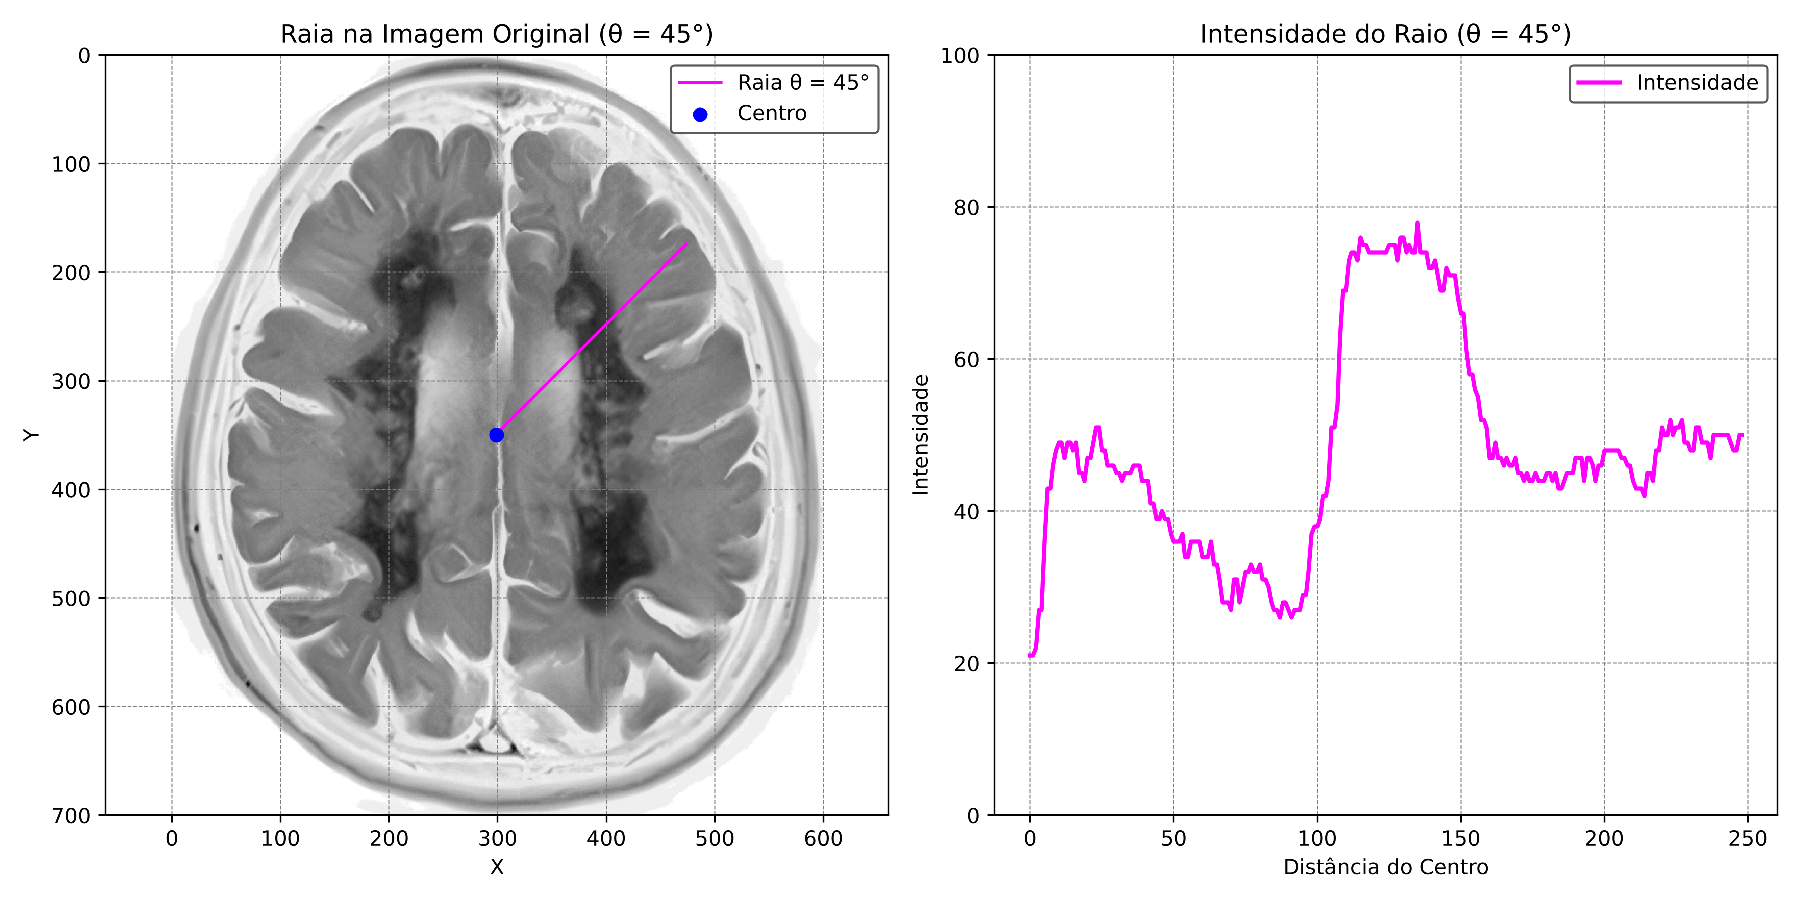
\includegraphics[width=1\linewidth]{./Figures/inverted_instance.pdf}
	\label{fig:perfil_de_intensidade}
\end{figure}

Essa formalização permite que os vetores propostos sejam facilmente operados em um espaço vetorial de dimensão finita $\mathbb{R}^N$, o que garante automaticamente a completude do espaço, tornando as operações lineares triviais. Contudo, é importante denotar que o uso das informações radiais para treinamento já constitui uma forma de aglutinação de dados e redução da dimensionalidade do sistema, que pode e será instrumentalizada para treinamento de modelos e testes comparativos. 

Visto isso, algumas operações vetoriais triviais sobre esse espaço podem ser definidas. A seguir, estão apresentadas, respectivamente, a intensidade média ($\hat{O}$), simetria ($\hat{S}$) e a simetria quiral ($\hat{\chi}$): 
\begin{align}
	\hat{O} | \mathbf{v}_{\theta} \rangle &= \left( \frac{1}{N} \sum_{k=1}^N I(r_k, \theta) \right) | \mathbf{v}_{\theta} \rangle, \\
	\hat{S}\, |\mathbf{v}_\theta\rangle &= \langle \mathbf{v}_\theta | \mathbf{v}_{-\theta}\rangle\, |\mathbf{v}_\theta\rangle, \\
	\hat{\chi}\, |\mathbf{v}_\theta\rangle &= \sum_{\theta'} \Big| \langle \mathbf{v}_\theta | \mathbf{v}_{\theta'}\rangle - \langle \mathbf{v}_{-\theta} | \mathbf{v}_{-\theta'}\rangle \Big|\, |\mathbf{v}_\theta\rangle.
	\label{eq:chi}
\end{align}
Cada um desses operadores mede uma quantidade e incorpora ela ao próprio estado, atuando como um filtro, gerando novos conjuntos vetoriais de mesma base que preservam as informações originais do estado, como a direção angular. Logo, todos esses resultados são passíveis da avaliação de correlação e densidade angular. Dito isso e com base na aplicação dos operadores, a concatenação de operações vetoriais permite a {\lq\lq}releitura do problema{\rq\rq}, levantando questionamentos como: qual seria o perfil de simetria das relações de intensidade média angular? Mostrando o quão versátil é a abordagem para criação de identidades relacionadas a diferentes anomalias, tanto as diretamente aferíveis, como as elusivas.
\begin{figure}[t!]
	\centering
	\caption{Operadores $\hat{O}$, $\hat{S}$ e $\hat{\chi}$ aplicados ao conjunto de vetores radiais $| \mathbf{v}_{\theta} \rangle$, para a imagem seccional observada na Figura \ref{fig:perfil_de_intensidade}. Estão plotadas as comparações entre a simetria e sua versão quiral, assim como os dados de intensidade média, ambos mediante variação angular.}
	\vspace{0.5cm}
	\begin{minipage}{0.45\textwidth}
		\centering
		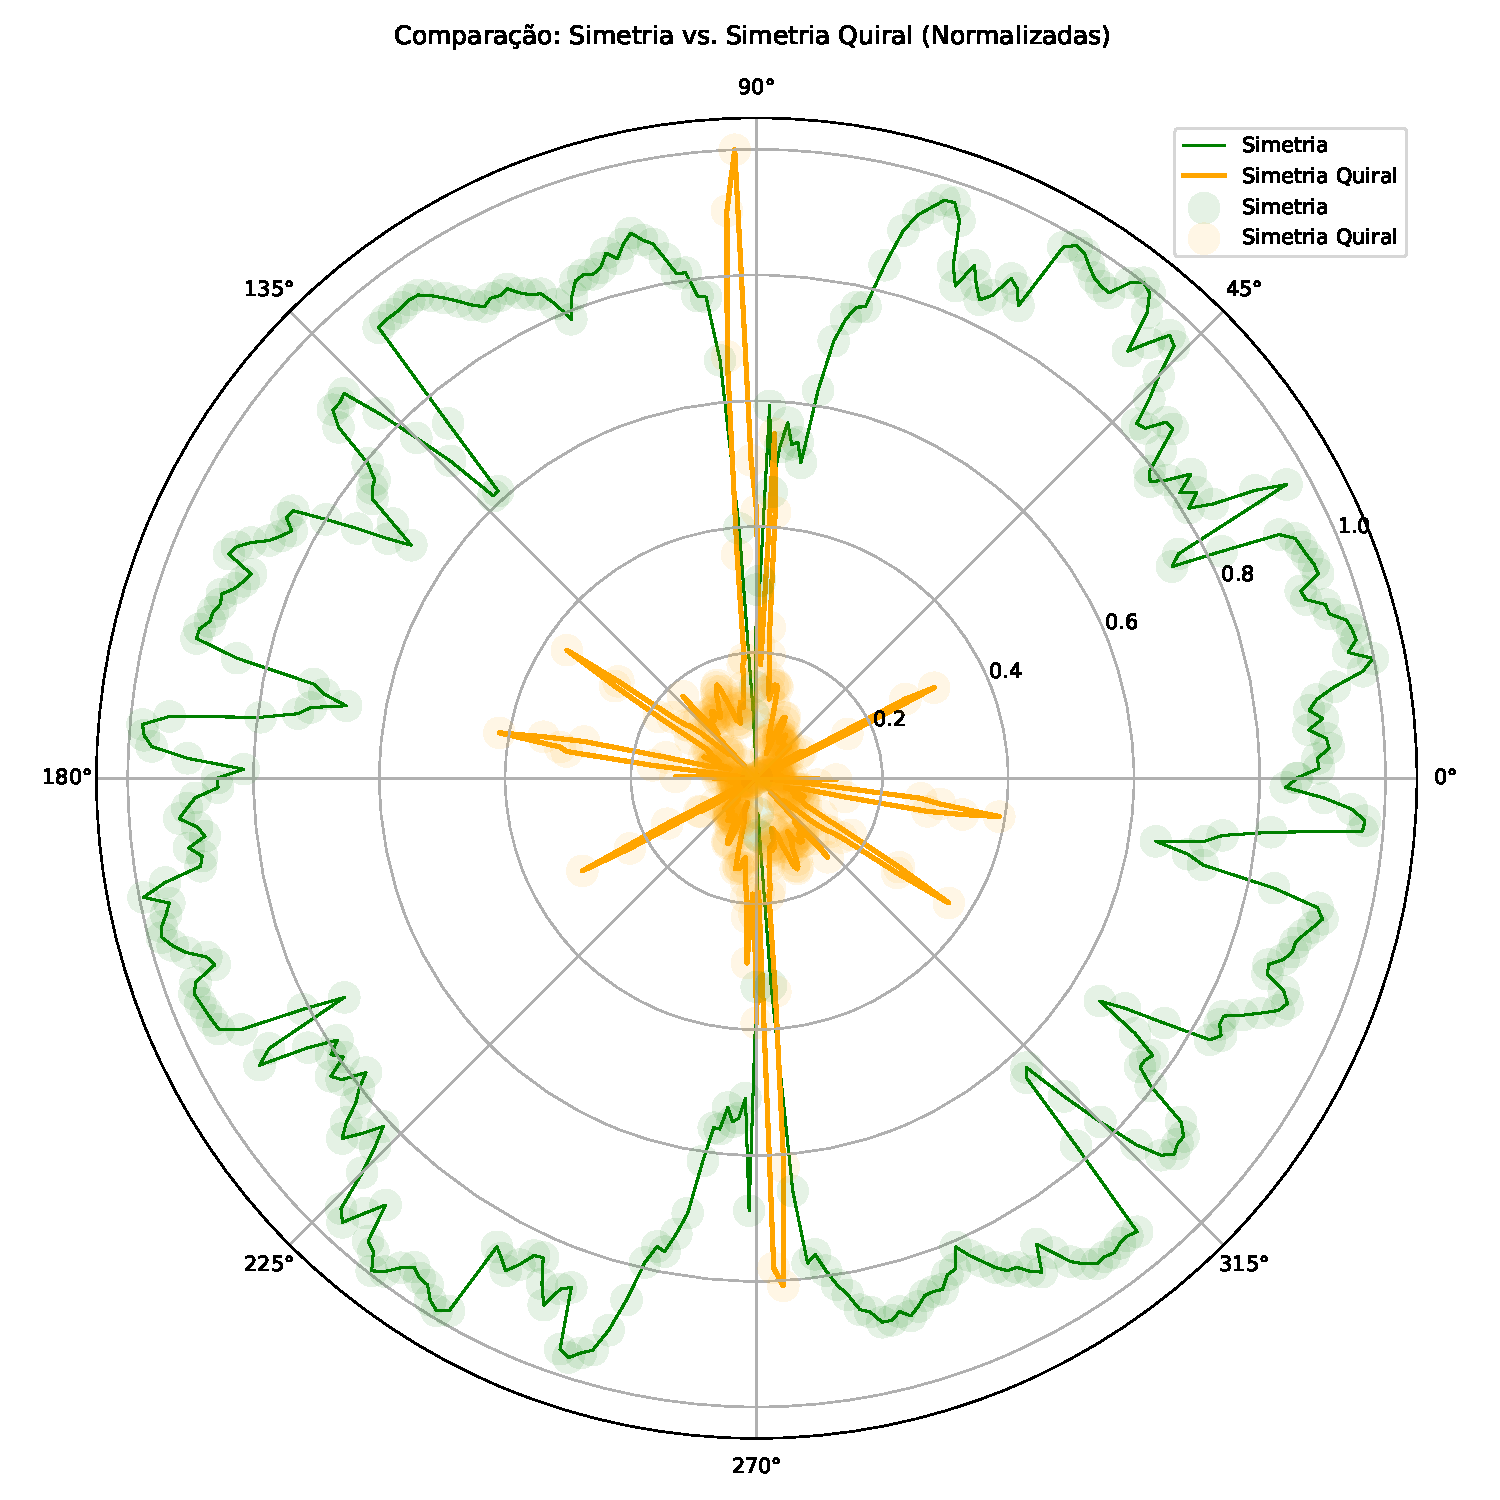
\includegraphics[width=1\linewidth]{./Figures/combined_symmetry_chiral_polar_normalized.pdf}
		\label{fig:combined_symmetry_chiral_polar_normalized}
	\end{minipage}
	\hfill
	\begin{minipage}{0.49\textwidth}
		\centering
		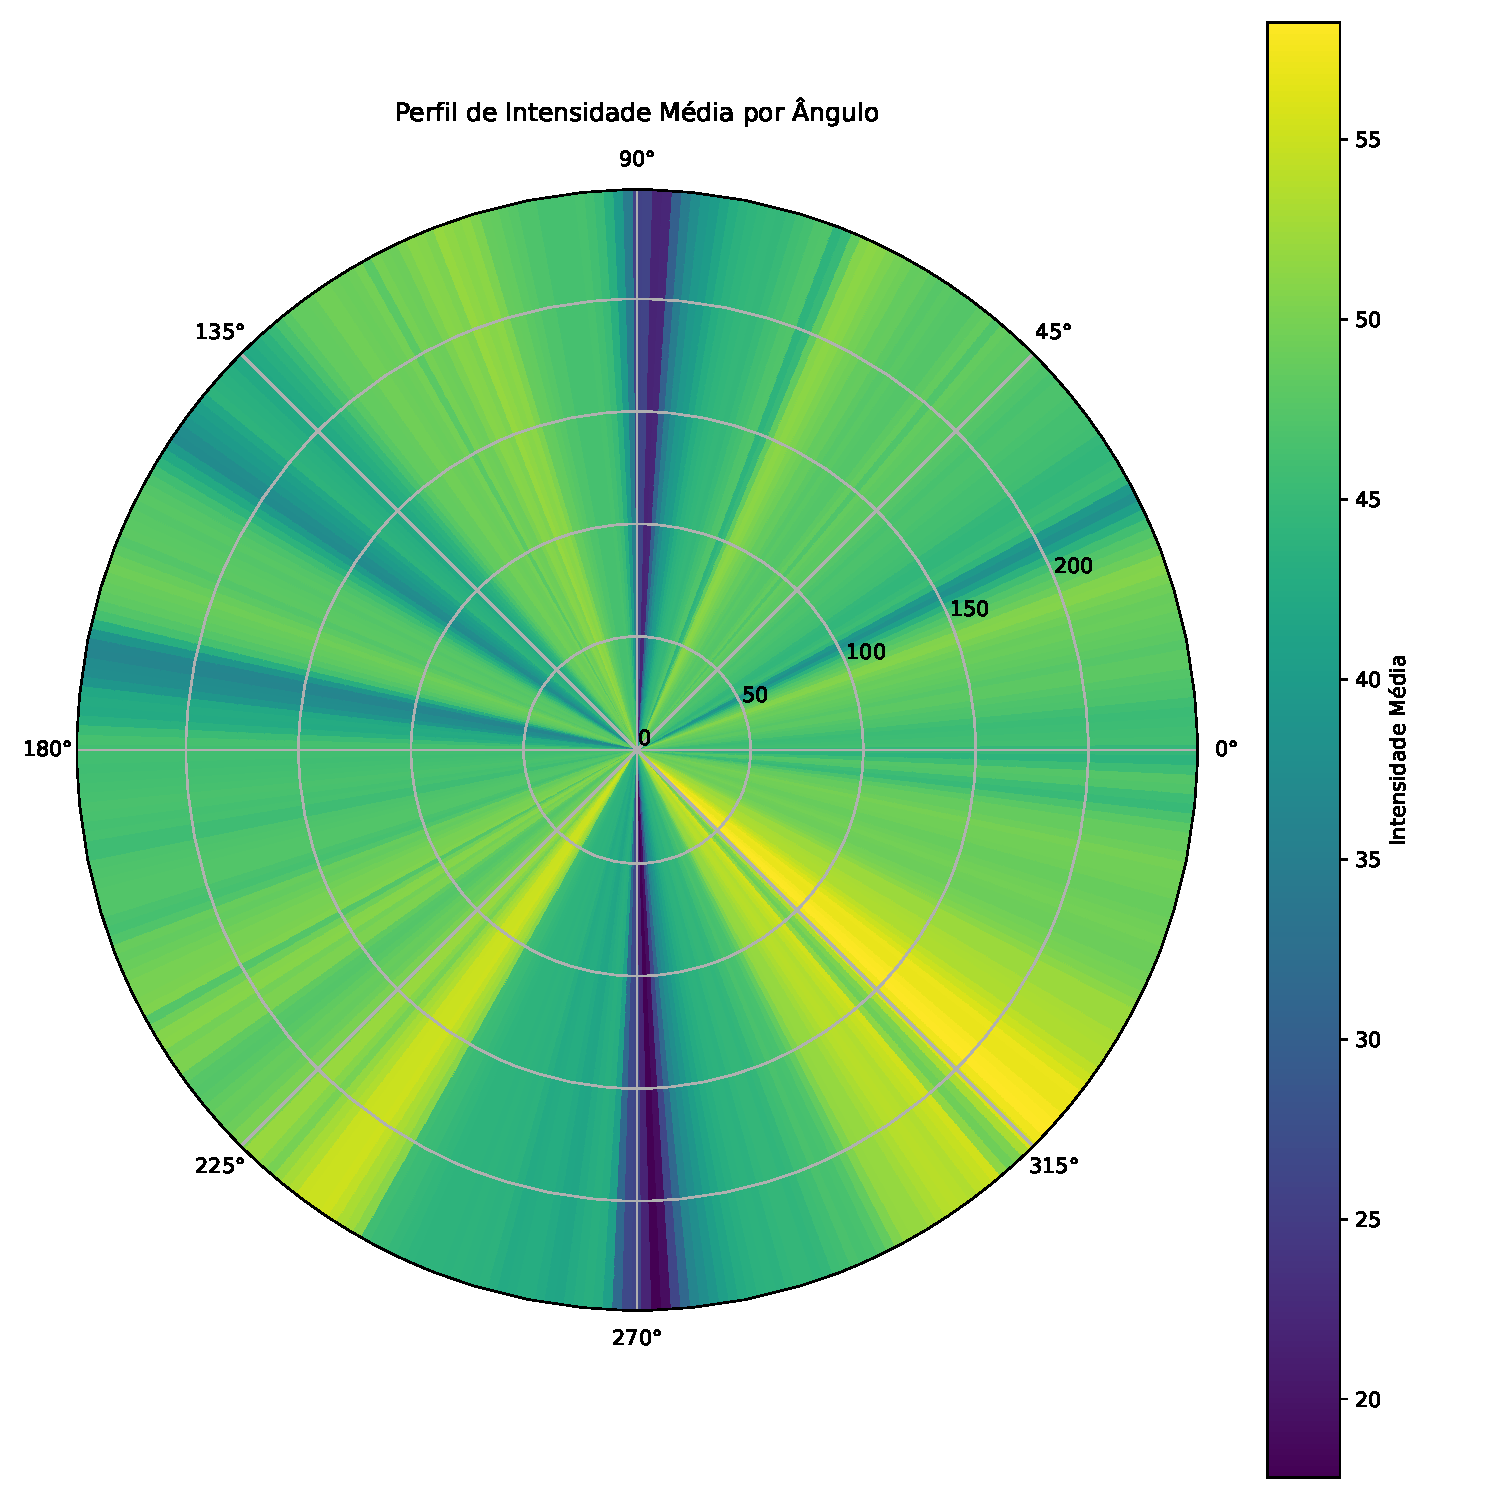
\includegraphics[width=1\linewidth]{./Figures/mean_intensity_profile.pdf}
		\label{fig:mean_intensity_profile}
	\end{minipage}

	\label{fig:primeiros_operadores}
\end{figure}

A Figura \ref{fig:primeiros_operadores} mostra o comportamento concatenado dos operadores de simetria e simetria quiral. Quando observada em conjunto com a Figura \ref{fig:perfil_de_intensidade}, constata-se claramente como a componente quiral denota a presença de anomalia e suas correlações angulares. As mesmas observações são transpostas para o perfil de intensidade média angular, na forma de variações abruptas de intensidades subsequentes. É interessante observar que mesmo anomalias não aparentes podem mudar levemente as correlações esperadas e, consecutivamente, gerar picos proeminentes nesses indicadores ou variações na estrutura normal esperada.

\begin{figure}[t!]
	\centering
	\caption{Operadores $\hat{D}$ e $\hat{R}$ aplicados ao conjunto de vetores radiais $| \mathbf{v}_{\theta} \rangle$, para a imagem seccional observada na Figura \ref{fig:perfil_de_intensidade}. A versão recíproca está em base $| \mathbf{e}_k \rangle$, logo, não se sobrepõem diretamente aos dados originais, enquanto a versão diferencial apresenta coesão direta.}
	\vspace{0.5cm}
	\begin{minipage}{0.48\textwidth}
		\centering
		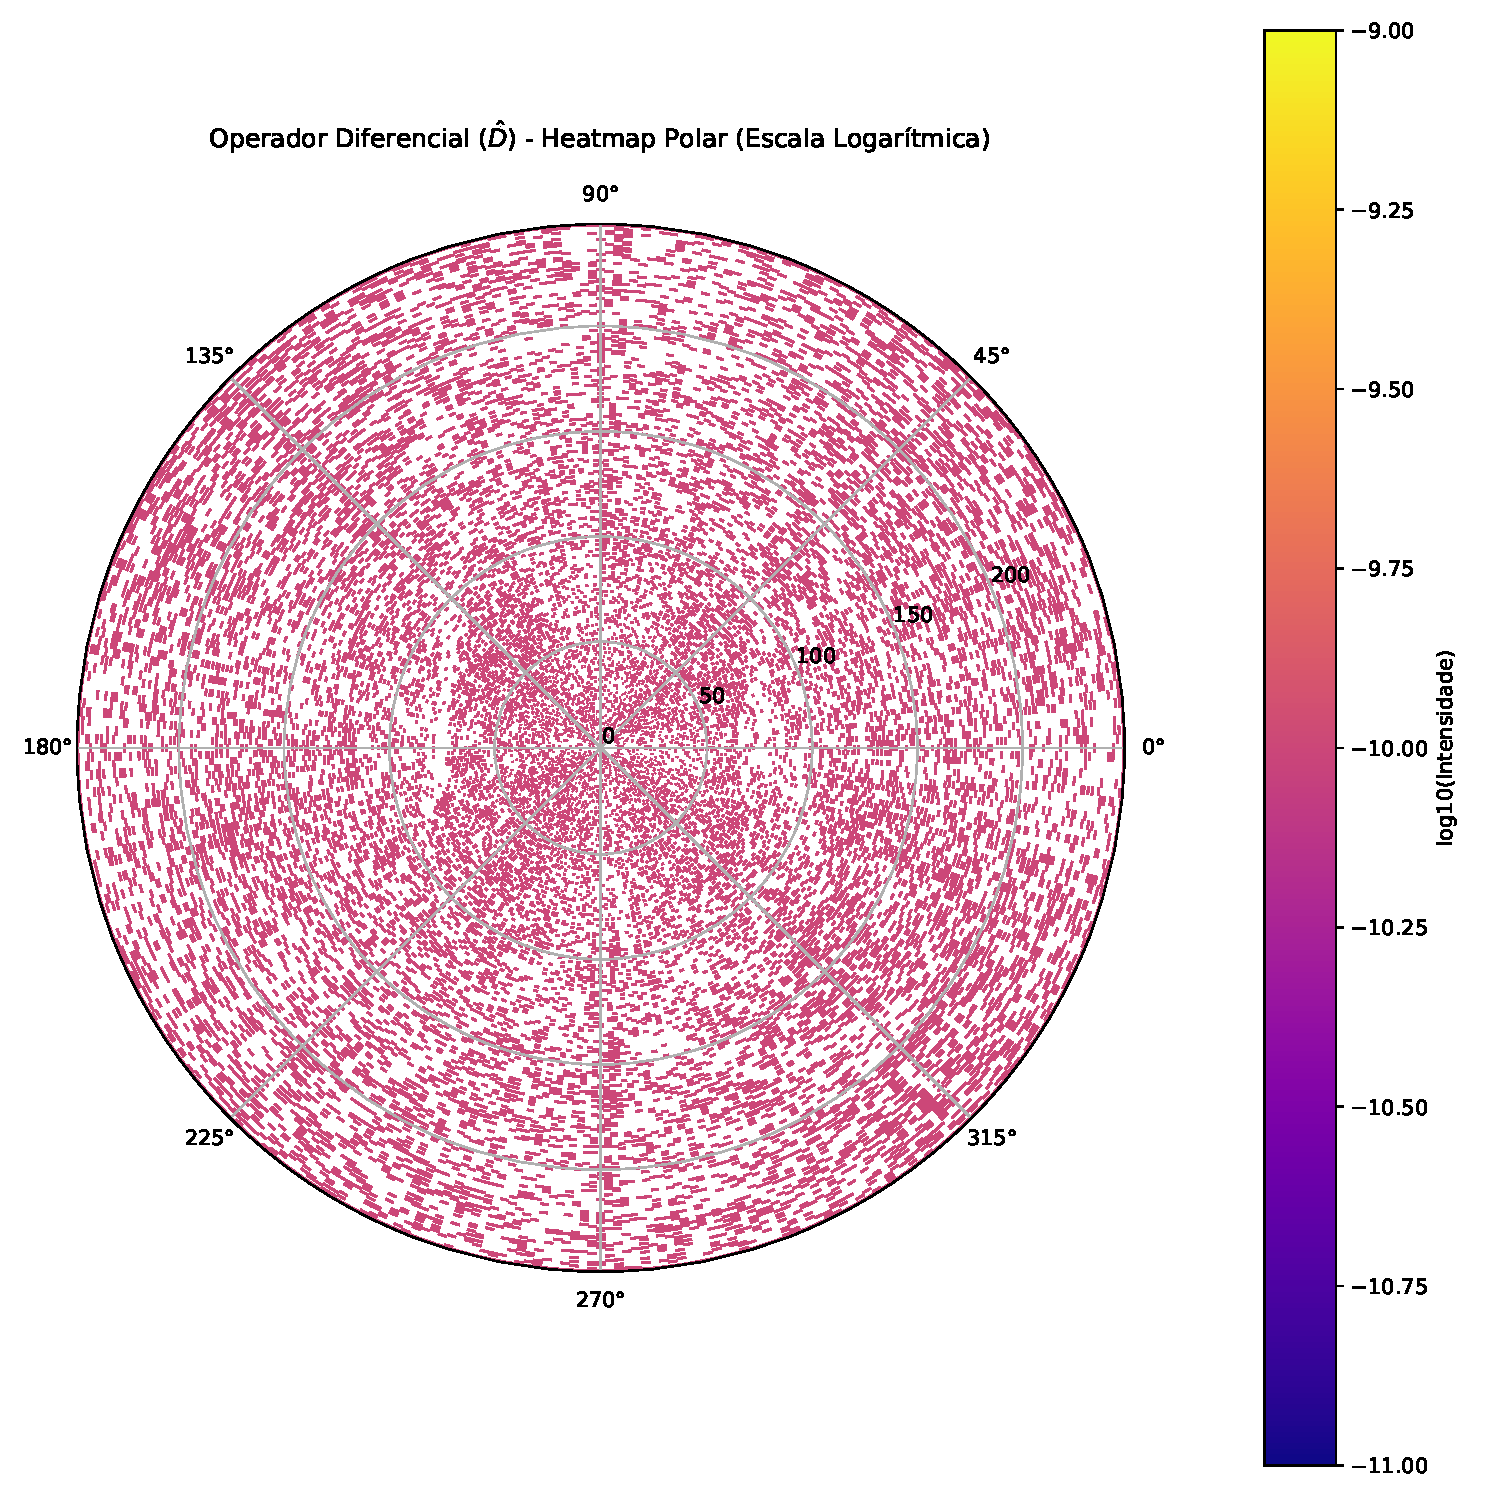
\includegraphics[width=1\linewidth]{./Figures/differential_operator_polar_heatmap_log.pdf}
		\label{fig:D}
	\end{minipage}
	\hfill
	\begin{minipage}{0.48\textwidth}
		\centering
		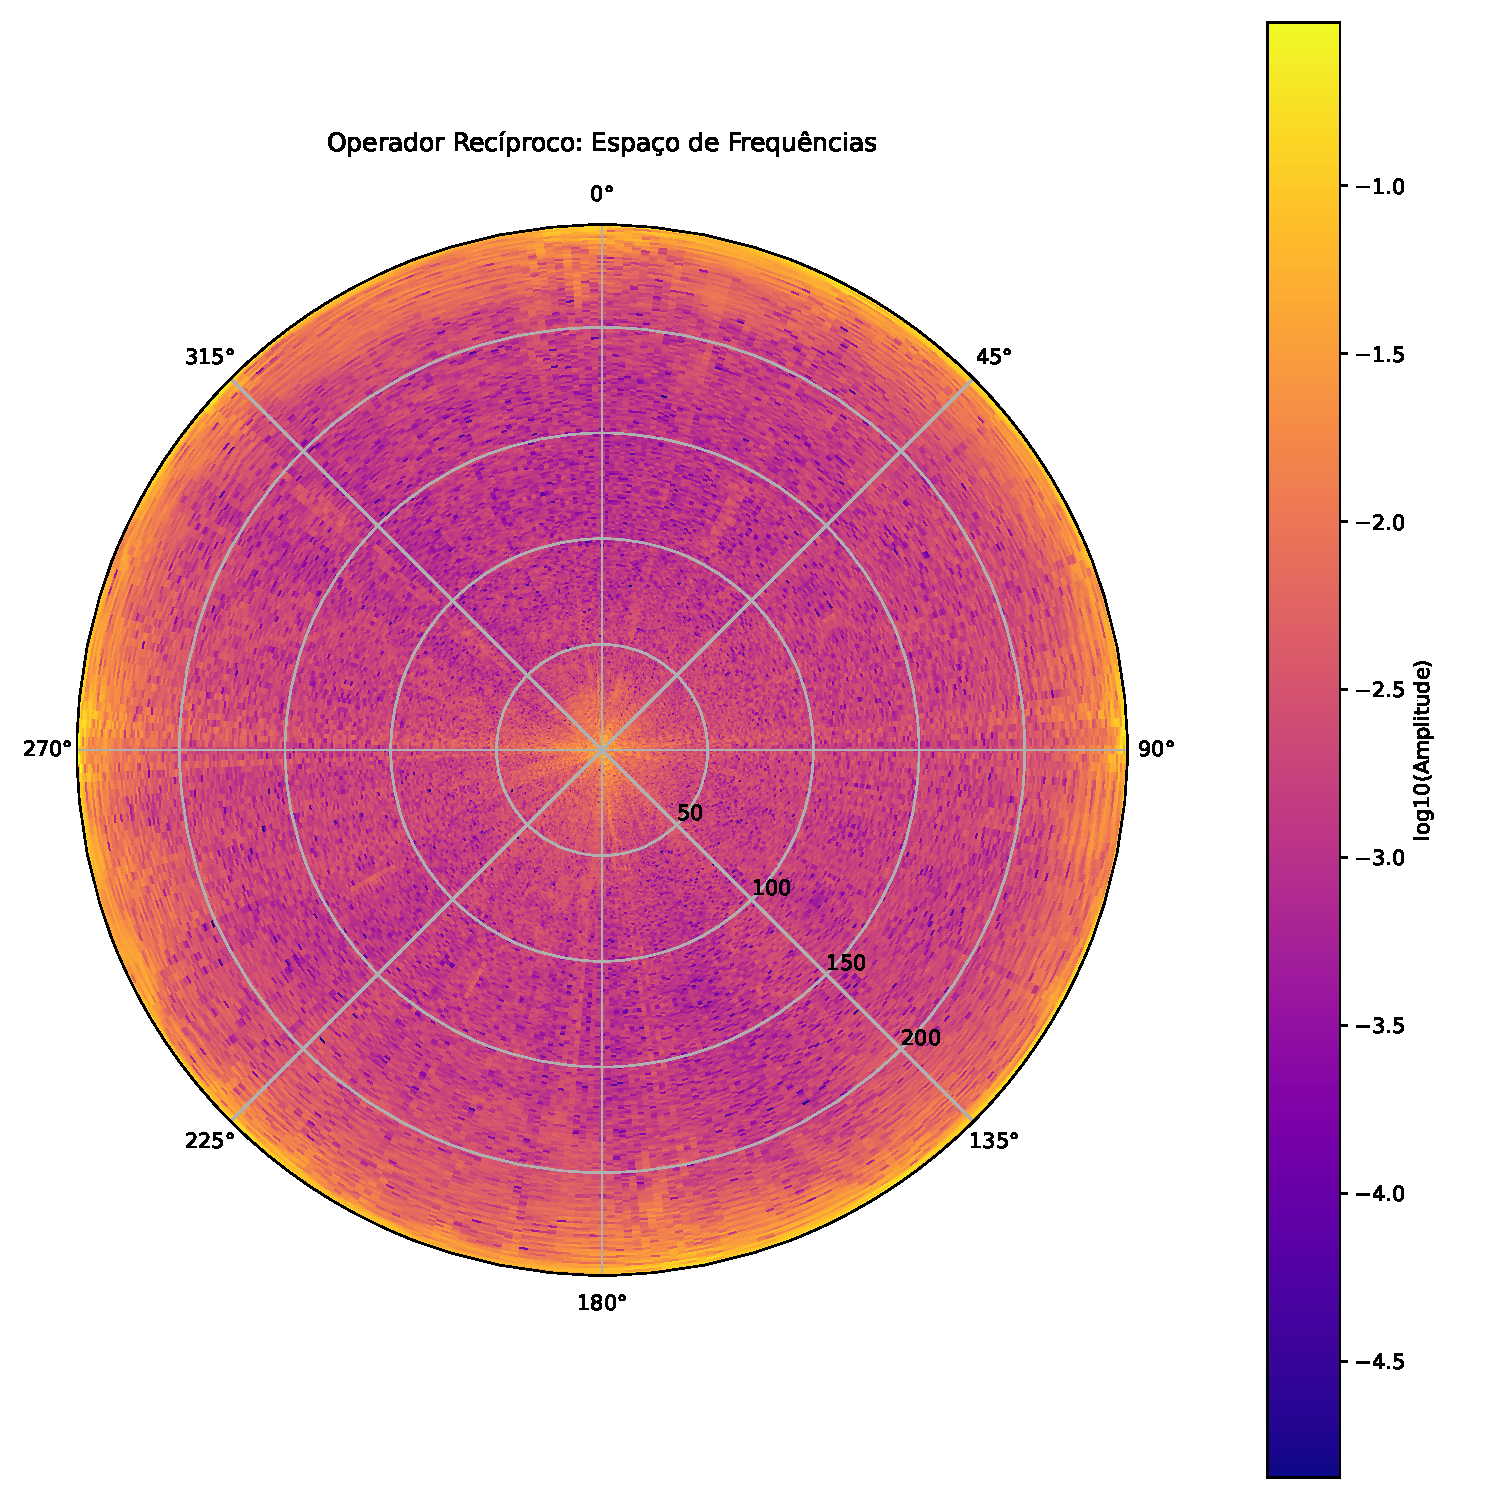
\includegraphics[width=1\linewidth]{./Figures/reciprocal_operator_full_spectrum.pdf}
		\label{fig:R}
	\end{minipage}
	
	\label{fig:DeR}
\end{figure}

Como o espaço proposto é finito em $\theta$, uma relação inspirada na resistência diferencial\footnote{Conceito oriundo da classificação de fases dinâmicas em sistemas caóticos de $n$-partículas de interação mútua repulsiva \cite{Mizrahi2002}.} pode ser equacionada com a utilização de diferenças finitas sobre ângulos adjacentes. Com isso, um operador que denota a transição de zonas é delimitado, evidenciando mudanças de tecido nos perfis radiais, assim como deformações não esperadas. Nessa abordagem a constância é planificada, enquanto a variação gera uma inflexão, substancialmente elevada pela imposição da escala logarítmica. Desse modo, o operador diferencial ($\hat{D}$) pode ser equacionado, como:
\begin{align}
	\hat{D} | \mathbf{v}_\theta \rangle = \left( \sum_{k=1}^{N-1} \ln \left| \frac{I(r_{k+1}, \theta) - I(r_k, \theta)}{\Delta r} \right| \right) | \mathbf{v}_\theta \rangle.
	\label{eq:D}
\end{align}

Muito embora ainda simples, mas de interpretação menos trivial, o conjunto vetorial pode ser levado ao espaço recíproco, uma vez que ele é bem definido sobre o real ($\mathbb{R}^N$). Nessa transposição espacial, as relações de comensurabilidade mútua entre os $n$ vetores radiais são evidenciadas. Para isso, a transformada discreta de Fourier é aplicada nos perfis radiais $ I(r, \theta)$. Sabendo que $X(k)$ é a contribuição normalizada da frequência associada ao índice $k$, as relações podem ser escritas:
\begin{align}
	X(k) &= \frac{1}{\sqrt{N}} \sum_{r=1}^N I(r, \theta) e^{-i \frac{2\pi}{N} (k-1)(r-1)}, \\
	\hat{R} | \mathbf{v}_\theta \rangle &= \sum_{k=1}^N X(k) | \mathbf{e}_k \rangle, \\
	\hat{R} | \mathbf{v}_\theta \rangle &= \sum_{k=1}^N \left( \frac{1}{\sqrt{N}} \sum_{r=1}^N e^{-i \frac{2\pi}{N} (k-1)(r-1)} I(r, \theta) \right) | \mathbf{e}_k \rangle.
	\label{eq:R}
\end{align}

É bastante razoável pressupor que os resultados desses operadores sejam menos palatáveis do que os anteriores, contudo, basta olhar atentamente para as características que eles impuseram sobre o espaço vetorial para que se constate o quão apreciáveis elas são para detecção automatizada via treinamento de redes neurais. Esse é o motivo pelo qual foi denotado o resultado da aplicação dos operadores como {\lq\lq}construtos virtuais{\rq\rq}, pois são abstrações obtidas sobre o espaço real que fornecem uma visão particular segundo sua prescrição.   

O operador $\hat{D}$, visto na Figura \ref{fig:DeR}, gera uma rede de picos que separam os tecidos, logo sua morfologia não é aleatória, mas sim produto direto da estrutura original. É aceitável que existam variações entre o esperado dessa estrutura para diferentes indivíduos, contudo, uma análise sobre os parâmetros que formam essa estrutura seguramente mantém constância para indivíduos que não apresentam anomalias. Aferições podem ser tomadas pela constituição de uma nova rede, onde um anel é expandido simultaneamente em cada ponto da rede original, até que esses anéis se encontrem e colidam, formando um padrão com certa regularidade, a estrutura gerada seria passível de métricas de ordem, coesão e classificação topológica \cite{Kittel1965}. É também interessante lembrar que $\hat{D}$ pode ser tomado sobre os resultados de $\hat{O}$, o que gera uma distribuição menos densa e mais comportada\footnote{Devido ao escopo reduzido do presente projeto, optou-se por evitar aplicações recorrentes de operadores.}.

Já o operador $\hat{R}$, presente na Figura \ref{fig:DeR}, cria um perfil onde as informações referentes à ordem da cada raio se traduzem em frequências. Por razão dessa característica, as estruturas de baixa frequência de cada perfil radial são relacionadas à morfologia ordinária, enquanto variações de alta frequência podem ser indicativos de anomalias, principalmente quando todo perfil radial é estudado. Esse operador apresenta, por natureza, maior expectativa de conformidade entre amostras não anômalas. É preciso frisar que uma discussão sobre as condições de contorno e fronteira do problema é requerida, como é facilmente observável pelo comportamento da intensidade visto nas bordas da Figura \ref{fig:DeR}, sendo essa uma casualidade típica da aplicação desse tipo de transformada nesses pontos característicos. Esse tópico será discutido melhor na seção seguinte.

$\frac{}{}$\\
\begin{Large}
	\textbf{3.2 Correlação Angular}
\end{Large}
$\frac{}{}$\\

Agora que o funcionamento do espaço vetorial foi elaborado, o comportamento da correlação angular pode ser definido e estudado. Se a correlação entre todos os perfis radiais for tomada, conectando matricialmente o resultado da permutação de todos os produtos internos radiais, a matriz $\text{C}_{\theta, \theta'}$ pode ser definida como $\text{C}_{\theta, \theta'} = \langle \mathbf{v}_\theta \,|\, \mathbf{v}_{\theta'} \rangle$ em $\mathbb{R}^{M\text{x}M}$, com $M$ raios. Além disso, verifica-se que $\text{C}_{\theta, \theta'}$ contempla três requisitos por consequência da definição do produto interno: é positiva, simétrica (logo $\text{C}_{\theta, \theta'} = \text{C}_{\theta', \theta}$) e possui diagonal unitária $\text{C}_{\theta, \theta} = 1$.

\begin{figure}[t!]
	\centering
	\caption{Autovalores ($\lambda_i$) e autovetores ($|u_i\rangle$) de $\hat{C}$, para a imagem seccional observada na Figura \ref{fig:perfil_de_intensidade}. Foi utilizado o conceito de {\lq\lq}informação{\rq\rq} para apresentar o significado de $\lambda_i$. Os autoestados plotados são os três de maior relevância.}
	\vspace{0.5cm}
	\begin{minipage}{0.45\textwidth}
		\centering
		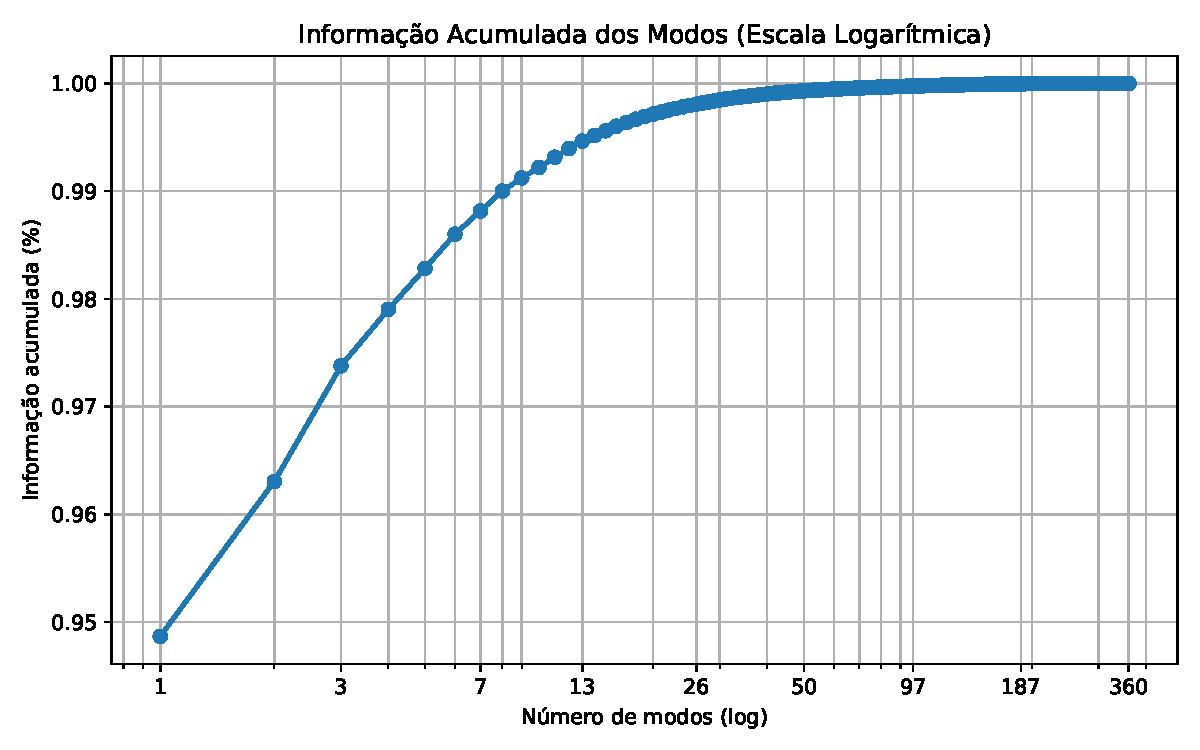
\includegraphics[width=1\linewidth]{./Figures/energy_accumulated_log.pdf}
		\label{fig:Aval}
	\end{minipage}
	\hfill
	\begin{minipage}{0.49\textwidth}
		\centering
		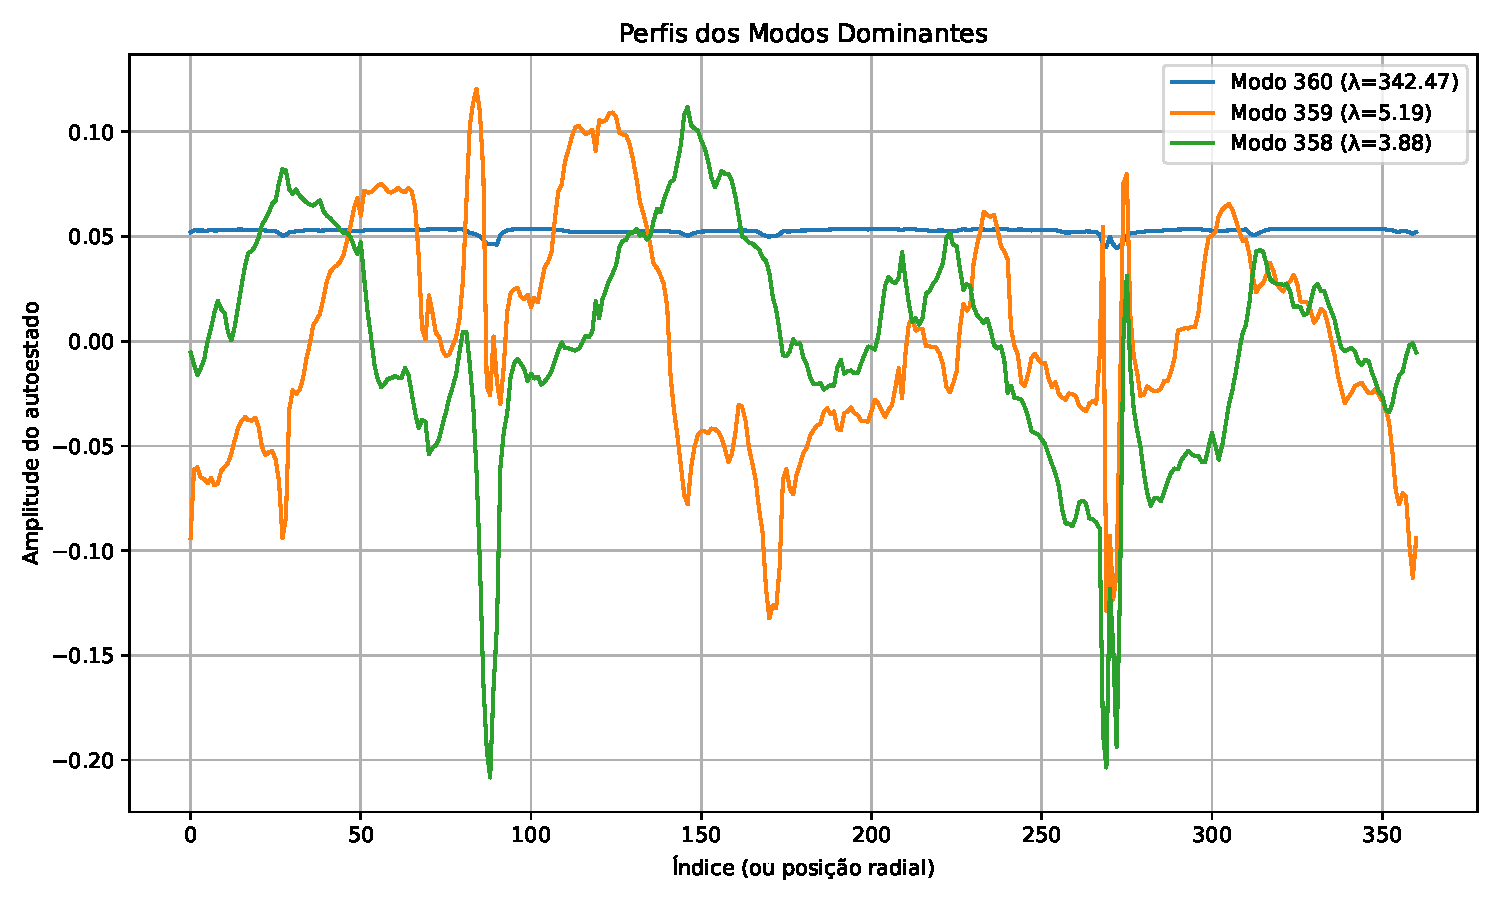
\includegraphics[width=1\linewidth]{./Figures/modes_profiles.pdf}
		\label{fig:Avec}
	\end{minipage}
	
	\label{fig:C_Aval_Avec}
\end{figure}

De modo resumido, $\text{C}_{\theta, \theta'}$ contempla todas as combinações lineares possíveis dos perfis angulares. Com isso, um operador linear pode ser definido com o propósito de agregar todas as combinações dos perfis radiais obtidos sobre os vetores $| \mathbf{v}_\theta \rangle$,
\begin{align}
	\hat{C}\ | \mathbf{v}_\theta \rangle = \sum_{\theta' = 1}^{M} \langle \mathbf{v}_\theta \,|\, \mathbf{v}_{\theta'} \rangle \, | \mathbf{v}_{\theta'} \rangle.
	\label{eq:C}
\end{align}
Felizmente, o Teorema Espectral permite resolver qualquer operador simétrico, ou matriz simétrica, através da diagonalização e decomposição de seus autovalores ($\lambda_i$) e autovetores ($|u_i\rangle$) a eles correspondentes. Nesse contexto, a análise pode ser simplificada como: $\hat{C} \, |u_i\rangle = \lambda_i \, |u_i\rangle$; com isso os autovalores atuam como um fator de escala, que demonstra a importância do papel de cada um dos modos, codificados  nos autovetores $|u_i\rangle$. Como esse espaço é ortogonal, cada vetor $|u_i\rangle$ é único, ou seja, o produto interno entre esses vetores é nulo, logo cada contribuição unitária apresenta uma perspectiva singular do todo.

Os modos podem ser entendidos como as componentes geométricas intrínsecas que compõem o objeto de estudo. Não somente isso, os modos podem ser remapeados para o espaço real original dos vetores radiais $|\mathbf{v}_\theta \rangle$. Com isso, o objeto de estudo pode ser reconstruído com base na combinação linear dos modos dominantes, segundo a equação:   
\begin{align}
	\hat{C}_{\text{reconstruída}} = \sum_{i=1}^K \lambda_i |u_i\rangle\langle u_i|.
	\label{eq:CparaR}
\end{align}

A Figura \ref{fig:C_Aval_Avec} mostra um resultado bastante curioso quando a contribuição dos modos para a informação total do objeto de estudo é mensurada. Quase 95\% de toda a informação que compõe a imagem está situada em apenas um único modo, que, com base na Equação \ref{eq:CparaR}, pode ser reconstruído e visualizado, como visto na Figura \ref{fig:modos}. Outra observação é a baixa variância apresentada pelo autoestado correspondente ao modo dominante, o que o torna um candidato ideal para instrumentalização como parâmetro de classificação. Conceituam-se, então, novos {\lq\lq}construtos virtuais{\rq\rq} delimitados, que serão instrumentalizados para detecção de anomalias por meio de redes neurais.

\begin{figure}[t!]
	\centering
	\caption{Utilização da Equação \ref{eq:CparaR} para reconstituição dos três  modos dominantes observados na Figura \ref{fig:C_Aval_Avec} no espaço real radial original.}
	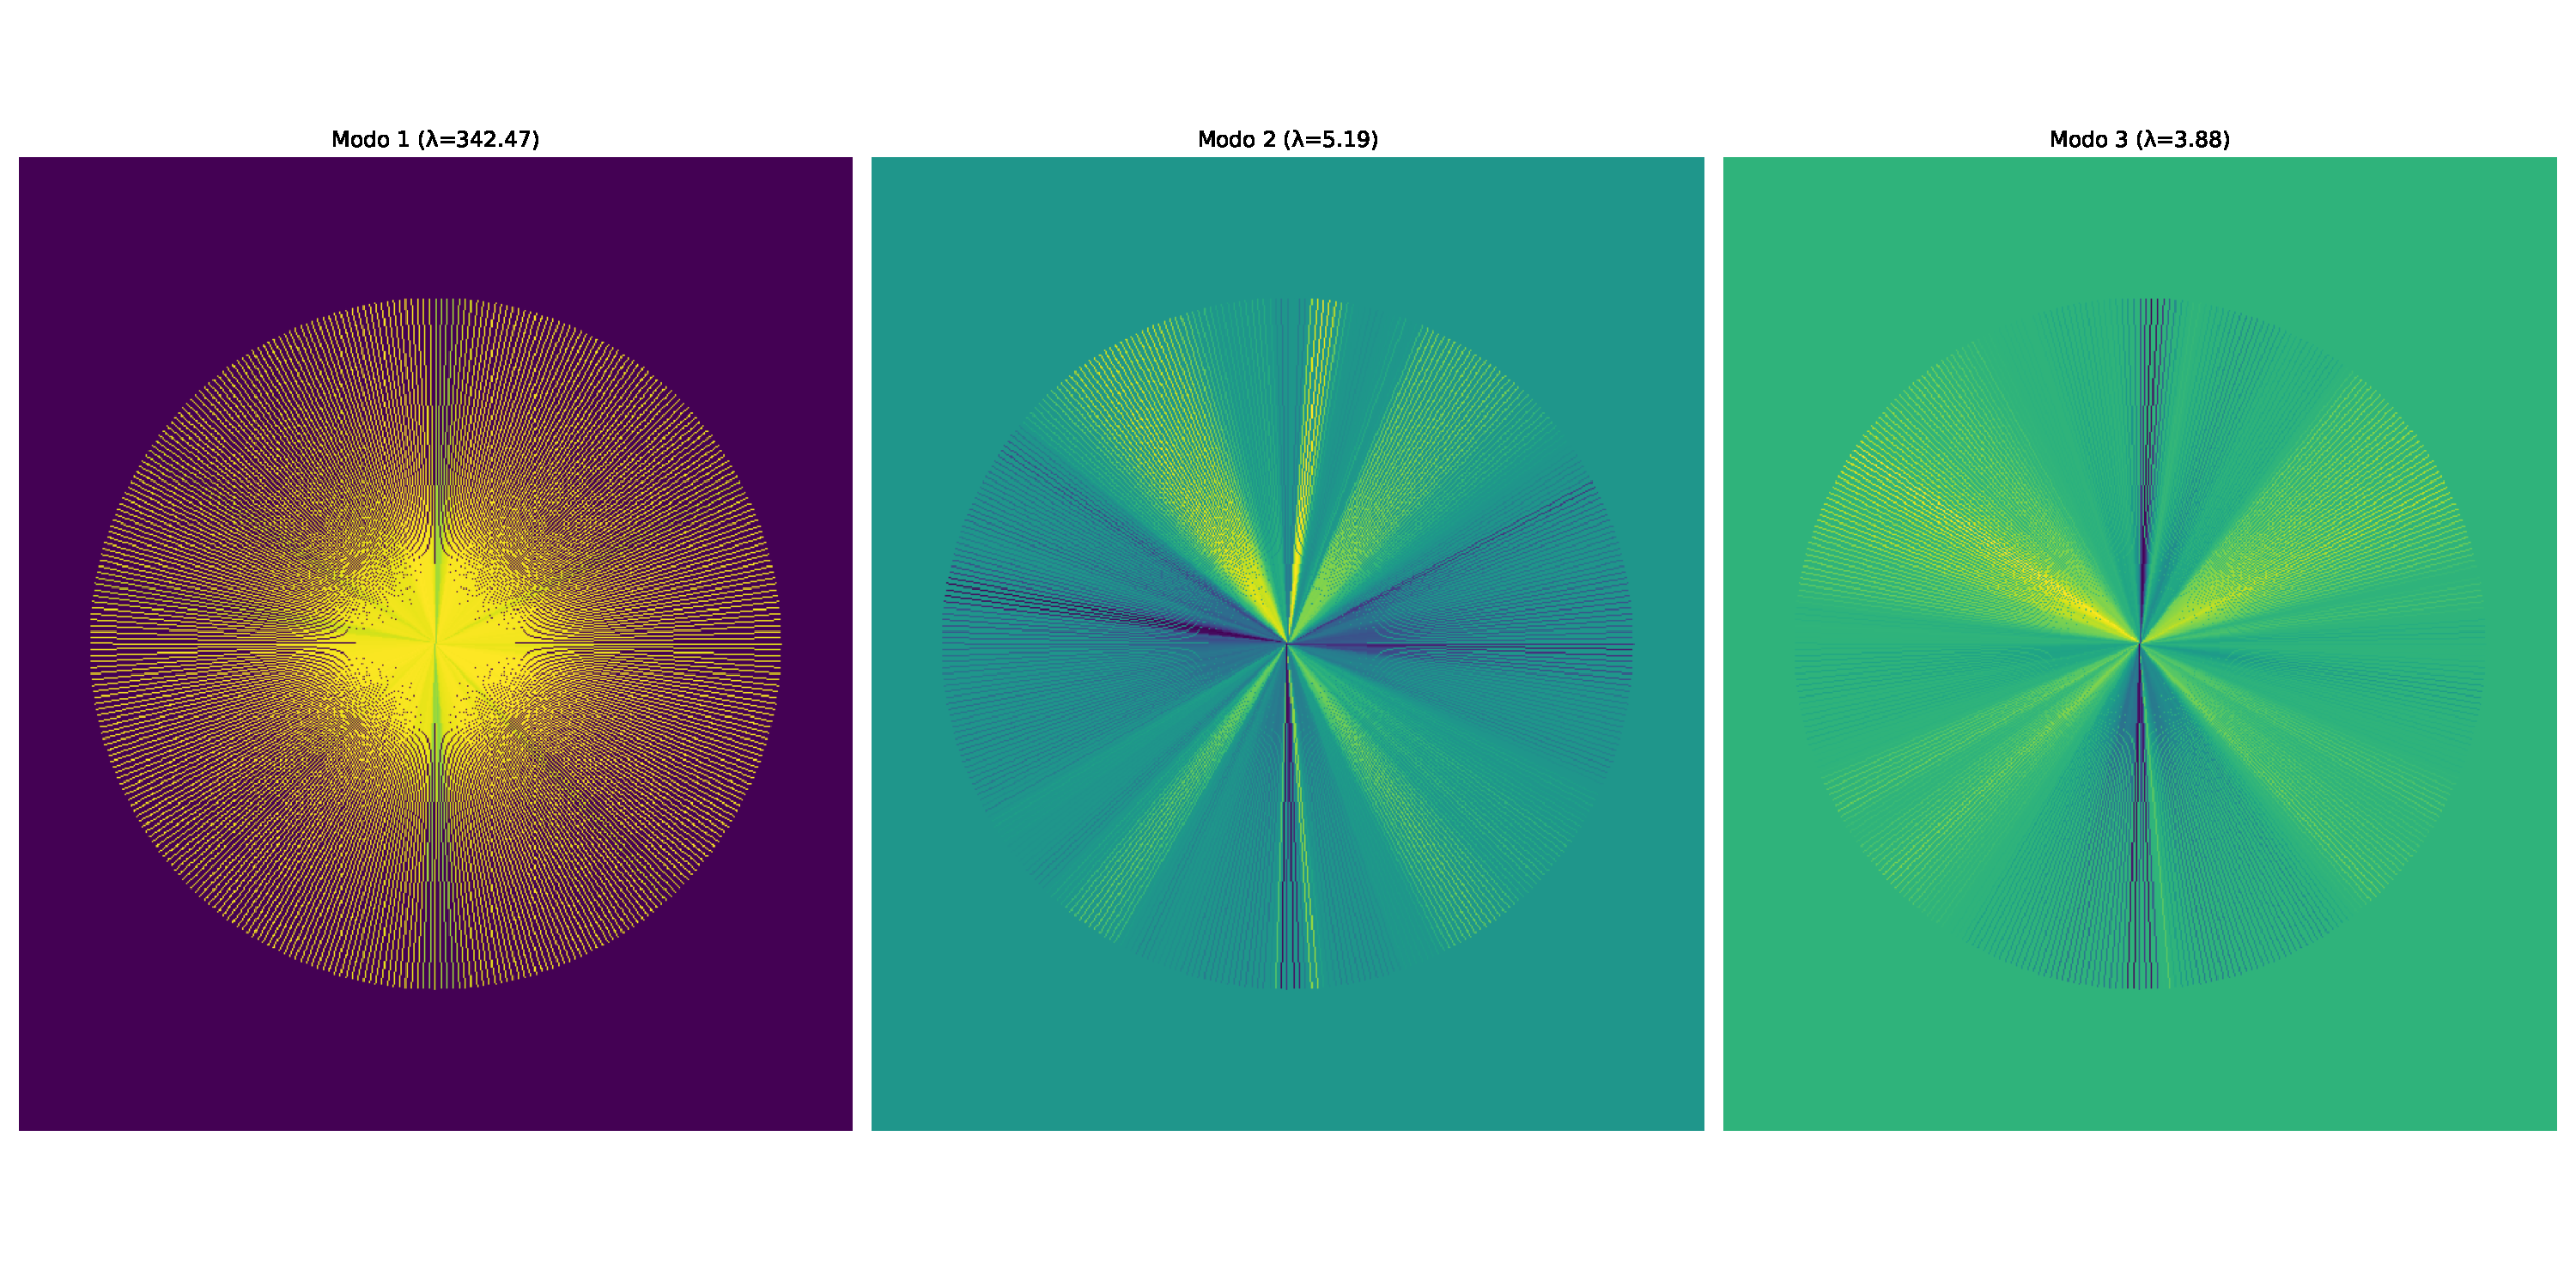
\includegraphics[width=1\linewidth]{./Figures/dominant_modes_images.pdf}
	\label{fig:modos}
\end{figure}

Durante a execução desse projeto, o raio foi truncado para evitar a discussão da condição de contorno, que será investigada durante a execução do mesmo. É possível que a adição \textit{ad-hoc} de uma fronteira que atue como {\lq\lq}anteparo de onda{\rq\rq} ajude a estabilizar os modos. A razão de tal consideração se dá em decorrência da excentricidade do crânio, que gera zonas vazias na coleta angular, podendo gerar um pequeno {\lq\lq}vazamento{\rq\rq} dos modos, dificultando a comparação. Contudo, se necessário, isso pode ser facilmente solucionado com a adição de uma condição de contorno anelar.

O formalismo vetorial enunciado pode ser aplicado para estudo dos vetores de diferentes planos, não somente isso, mas uma consistência entre os modos é esperada, ou seja, quebras nessa expectativa podem indicar a presença de anomalias, tanto observáveis quanto elusivas. Métrica esta que também será instrumentalizada.

Por fim, é importante lembrar que apenas alguns dos muitos possíveis operadores sobre o espaço foram enunciados. Efetivamente, o formalismo apresentado permite a translação direta de toda uma bibliografia voltada ao estudo da matéria para o estudo de informações em imagens de MRI ou submetidas a imposição de simetria radial. Denota-se ainda que, tudo aqui proposto se assemelha a constituição de uma técnica de PCA \cite{JolliffePrincipal2016Apr}, porém estritamente desenvolvida para estudo e classificação de anomalias em imagens pertencentes ao escopo estipulado.

$\frac{}{}$\\
\begin{Large}
	\textbf{3.3 Redes Neurais Convolucionais Clássicas.}
\end{Large}
$\frac{}{}$\\

Atualmente, o uso de redes neurais para obtenção de soluções complexas e não lineares tem se mostrado cada vez mais proeminente na literatura \cite{Iqbal2018, Kumar2023, Hays2024Dec,Binzagr2024Apr, Hussain2024,Mane2024}. Neste trabalho, será instrumentalizada a coesão do formalismo já apresentado com Redes Neurais Convolucionais (CNN) \cite{Rawat2017,Khan2020, Li2021}, para obtenção de um resultado condizente entre os $n$ possíveis operadores.

Diferente das redes convencionais, onde parâmetros de peso ponderam cada neurônio da camada, redes convolucionais utilizam um conjunto de matrizes de peso ($\mathbf{W}_l$) para as chamadas {\lq\lq}operações de convolução{\rq\rq}. Essas operações consistem na aplicação de um operador linear que {\lq\lq}desliza{\rq\rq} sobre a matriz de parâmetros ingressante na camada, o que gera a extração de características do sistema, como a delineação de traços ou índices de profundidade em imagens. Nessas redes, a quantidade de matrizes de peso remete ao número de canais de saída ($c$) de cada camada ($l$). 

O funcionamento de CNNs pode ser separado em quatro etapas: convolução, redução de dimensionalidade, achatamento e resolução. Respectivamente, na primeira etapa, as matrizes de peso, usualmente chamadas de kernels, que produzem um mapa de características ao atuarem sobre a matriz de parâmetros, onde cada kernel produz um mapa distinto. Na segunda etapa, os dados são sumarizados e a dimensionalidade do problema é reduzida, essa operação é conhecida como \textit{Pooling}, onde a informação é preservada ao mesmo tempo que o conjunto de parâmetros é compactado, o que aumenta significativamente a eficiência computacional. Na etapa seguinte, o sistema de parâmetros passa por uma reestruturação, ou achatamento, e um vetor unidimensional e diretamente proporcional à escala da estrutura neural é obtido, esse vetor servirá como entrada para as camadas profundas. Por fim, a solução final é obtida por intermédio das camadas completamente conectadas, onde novas matrizes de peso ajustam a dimensionalidade do sistema em prol da constituição da saída desejada. É importante salientar que múltiplos objetivos podem ser almejados durante a resolução do sistema, de modo que, cada uma das camadas de solução é individualmente conectada aos canais de saída da última camada profunda.

Na Seção seguinte será apresentada a constituição da solução proposta por esse projeto em conjunto com a formulação de uma estrutura convolucional simples.

$\frac{}{}$\\
\begin{Large}
	\textbf{3.4 Espaço de Resoluções Condizentes}
\end{Large}
$\frac{}{}$\\

Essa proposta, objetivamente, engloba uma grande gama de possibilidades, discussões e análises. No entanto, isso não necessariamente é uma vantagem por si só, visto que, uma gama exorbitante de resultados arbitrários, mesmo que significativos, seria de difícil compreensão e contrariaria a demanda recente da literatura \cite{Zitu2024Dec,Hays2024Dec,Binzagr2024Apr}.

Com essa problemática em mente, é proposta a criação de um espaço dedicado à exposição dos resultados de modo condizente entre os múltiplos operadores e às $n$ observáveis identidades. Desse modo, toda proposta se solidifica em um único e coeso resultado, diretamente observável e mensurável, de compreensão trivial e desvinculado do formalismo laborioso utilizado. É proposto ainda que sua constituição seja produto natural do treinamento dos modelos, sem adição de especificações particulares.

Sendo assim, um espaço que apresente coesão comensurável ao Real ($1:1$) pode ser denominado, onde os resultados obtidos são mapeados para um plano, de modo que a visão {\lq\lq}ideal{\rq\rq} de um cérebro seria um plano perfeito, enquanto sua visão realista, de um cérebro saudável normal, se constitui de um plano com {\lq\lq}\textit{bumps}{\rq\rq}, ou seja, um relevo com solavancos de variações suaves. Para isso, duas regras básicas de constituição são denotadas: informações não locais versam diretamente sobre o \textit{ground-state}; enquanto informações locais se apresentam como uma perturbação gaussiana sobre o plano. Desse modo, a visualização desse resultado pode ser sobreposta à imagem original de secção, apresentando indícios e aferições sobre quaisquer tipos de anomalias, sejam elas, diretamente observáveis ou elusivas.     

Essa abordagem contempla e representa a resposta esperada de CNN, treinadas mediante ao procedimento descrito neste projeto. Tal congruência permite a observação da resolução de cada componente independente mediante a aplicação da superposição dos resultados individuais, propiciando a utilização desse resultado como candidato ideal de \textit{input} em redes profundas. Desse caminho em diante, é tomado como mais propício ao problema e a formalização apresentada, a busca pelas anomalias com base nas discrepâncias geradas por elas na estrutura ordinária, ou seja, será modelado o normal, detectando assim padrões atípicos frente ao esperado. Desse modo, a abordagem que se segue, foi elaborada para a utilização do modelo com dados não rotulados, mediante ao treinamento não supervisionado, o que já se mostrou promissor em trabalhos anteriores \cite{Mane2024,Nakao2021,Baur2021}.

Dadas as premissas apresentadas, a materialização das concepções pode ser obtida se, para cada pixel da imagem original, for posicionado o centro de uma Gaussiana em um plano de coordenadas ($x,y$). Neste projeto, será desprezado o tratamento da óbvia condição de contorno, que será tratada durante a execução do mesmo. Com isso, obtém-se uma malha 3D, oriunda da soma de $n$ Gaussianas \cite{Gaussian}, onde os pixels da imagem original $(i,j)$, são correlacionados à intensidade $\mathbf{Z}(x,y)$. Sendo ambas as imagens de mesma altura $H$ e comprimento $W$, pode-se equacionar:
\begin{align}
\mathbf{Z}(x,y) = \sum_{i=1}^H \sum_{j=1}^W A_{ij} \cdot \exp\left(-\frac{(x - i)^2 + (y - j)^2}{2\Sigma_{ij}^2}\right),
	\label{eq:Z(x,y)}
\end{align} 
onde os parâmetros $A_{ij}$ e $\Sigma_{ij}$ são, respectivamente, as matrizes de amplitude e variâncias, ambas positivas e não nulas\footnote{Na realidade, o caso particular de nulificação de $A_{ij}$ representaria a concepção de um cérebro ideal, um plano sem solavancos ou \textit{bumps}, logo, não observável por definição.}. Estes termos serão os resultados, \textit{outputs} de camadas convolucionais finais (\textit{heads} de saída). Para isso, uma estrutura convolucional simples será utilizada \cite{MartinAbadi2015}, como suas camadas convolucionais $\text{Conv2D}$ relacionadas aos canais de saída $\mathbf{F}_l$, responsáveis pela extração das características (\textit{features}), estruturadas do seguinte modo: 
\begin{align}
\mathbf{F}_1(i,j,c) &= \text{ReLU}(\text{Conv2D}(\mathbf{C}(i,j), \mathbf{W}_1)), \\
\mathbf{F}_2(i,j,c) &= \text{ReLU}(\text{Conv2D}(\mathbf{F}_1(i,j,c), \mathbf{W}_2)),
\end{align} 
onde $\text{ReLU}$ é a função de ativação não linear, aplicada na matriz $\mathbf{C}(i,j)$ ($i=1,…,H,j=1,…,W$), sendo $\mathbf{W}_1$ e $\mathbf{W}_2$ os conjuntos de \textit{kernels} utilizados na convolução. A notação de subíndice aqui remete à camada em si, logo essa operação refere-se ao que ocorrerá com todos os \textit{kernels} utilizados em cada camada, sendo o número desses elementos um parâmetro ajustável equivalente ao número de canais de saída $c$, com isso, anotação geral pode ser apresentada como:
\begin{align}
\mathbf{F}_l(i, j, c) = \text{ReLU}(\text{Conv2D}(\mathbf{F}_{l-1}, \mathbf{W}_l)).
\label{eq:Fl}
\end{align} 

Em sequência, uma camada de \textit{pooling} é aplicada com o propósito de reduzir a dimensionalidade das \textit{features}, enquanto preserva as informações originais. A função comumente utilizada nessa prática é chamada de $\text{MaxPooling}$, desse modo, pode-se tomar:
\begin{align}
	\mathbf{F}_3(i, j, c) &= \text{MaxPooling}(\mathbf{F}_2(i, j, c)).
	\label{eq:F3}
\end{align} 

Com isso, um vetor unidimensional de $k$ elementos e compacto em relação a $\mathbf{C}(i,j)$ é tomado e denominado como $\mathbf{h}_4$, em um procedimento conhecido como \textit{Flatten}. Curiosamente, $k$ é congruente ao número de neurônios por camada requeridos na constituição das camadas profundas. Desse modo, pode-se escrever:
\begin{align}
	\mathbf{h}_4 = \text{Flatten}(\mathbf{F}_3(i, j, c)),
	\label{eq:h4}
\end{align}
logo, com a adição de um novo vetor unidimensional de \textit{bias} $\mathbf{b}_l$, assim como a utilização de uma matriz de peso $\mathbf{W}_{l}^{bot}$, as camadas densas, conhecidas como \textit{bottleneck} podem ser apresentadas como:
\begin{align}
	\mathbf{h}_5 = \text{ReLU}(\mathbf{W}_{5}^{bot} . \mathbf{h}_4 + \mathbf{b}_5),
	\label{eq:h5}
\end{align}
desse modo, é gerada uma camada criada com o propósito de combinar todas as características obtidas do vetor compactado $\mathbf{h}_4$. Por fim, os \textit{heads} de saída podem ser obtidos e os parâmetros $A_{ij}$ e $\Sigma_{ij}$ apresentados na Equação \ref{eq:Z(x,y)} podem ser tomados. Para isso, será utilizada uma função \textit{Sigmoid} sobre $A_{ij}$, assim serão obtidas amplitudes diretamente normalizadas. Já para $\Sigma_{ij}$ será utilizada a função \textit{SoftPlus} ($\ln(1+\epsilon^x)$), resultando em variâncias positivas e não truncadas. Visto isso, com duas camadas densas e mutuamente independentes, obtém-se:
\begin{align}
	\mathbf{A}_6(i, j) = \text{Sigmoid}(\mathbf{W}_{6}^{out} \cdot \mathbf{h}_5 + \mathbf{b}_6),\\
	\mathbf{\Sigma}_7(i, j) = \text{Softplus}(\mathbf{W}_{7}^{out} \cdot \mathbf{h}_5 + \mathbf{b}_7).
	\label{eq:AeSigma}
\end{align}

\begin{figure}[t]
	\caption{Visualização da estrutura funcional da rede convolucional (CNN) proposta para obtenção dos parâmetros $A_{ij}$ e $\Sigma_{ij}$.}
	\vspace{0.6cm}
	\centering
	\resizebox{\textwidth}{!}{
		\begin{tikzpicture}[
			node distance=0.3cm and 0.8cm,
			latent/.style={draw, rounded corners, minimum width=3cm, minimum height=0.5cm, align=center, font=\small, text width=3.7cm},
			group/.style={draw, dashed, inner sep=0.4cm, rounded corners},
			arrow/.style={->, thick}
			]
	
	%% STACK 1: Entrada e Pré-Processamento
	%% STACK 1: Entrada e Pré-Processamento
	\node[latent, fill=blue!20] (coleta) {Entrada de Imagem Setorial \\ $\mathbf{I}(i,j)$};
	\node[latent, fill=blue!10, below=of coleta, text width=3.6cm] (transposicao) {Transposição e coleta Polar \\ $\mathbf{I}(r,\theta)$};
	\node[latent, fill=blue!10, below=of transposicao, text width=3.6cm] (entrada) {Entrada de componente resolvida, tal como: \\ $\mathbf{C} _{\theta,\theta '}$};
	\node[group, fit=(coleta) (transposicao) (entrada)] (grupo1) {};
	\node[above=0.1cm of grupo1.north] {\textbf{Aquisição}};
	
	%% STACK 2: F1, F2, F3
	% Posiciona stack 2 à direita da stack 1
	\node[latent, fill=green!20, right=2cm of coleta] (f1) {Convolução 1 \\ $l=1$ \\ $\mathbf{F}_1(i,j,c)$};
	\node[latent, fill=green!20, below=of f1] (f2) {Convolução 2 \\ $l=2$ \\ $\mathbf{F}_2(i,j,c)$};
	\node[latent, fill=green!20, below=of f2] (f3) {Pooling \\ $l=3$ \\ $\mathbf{F}_3(i,j,c)$};
	\node[group, fit=(f1) (f3)] (grupo2) {};
	\node[above=0.1cm of grupo2.north] {\textbf{Convolução}};
	
	%% STACK 3: Flatten, Bottleneck
	% Posiciona stack 3 à direita da stack 2
	\node[latent, fill=orange!20, right=2cm of f1] (flatten) {Flatten \\ $l=4$ \\ $\mathbf{h}_4$};
	\node[latent, fill=red!20, below=of flatten] (bottleneck) {Bottleneck \\ $l=5$ \\ $\mathbf{h}_5$};
	\node[group, fit=(flatten) (bottleneck)] (grupo3) {};
	\node[above=0.1cm of grupo3.north] {\textbf{Vectorização}};
	
	%% STACK 4: Heads de saída
	% Posiciona stack 4 à direita da stack 3
	\node[latent, fill=purple!20, right=2cm of flatten] (headAmp) {Head Amplitudes \\ $l=6$ \\ $\mathbf{A}_6(i,j)$};
	\node[latent, fill=purple!20, below=of headAmp] (headVar) {Head Variâncias \\ $l=7$ \\ $\mathbf{\Sigma}_7(i,j)$};
	\node[group, fit=(headAmp) (headVar)] (grupo4) {};
	\node[above=0.1cm of grupo4.north] {\textbf{Resolução}};
	
	%% Conexões entre as stacks
	% Uma seta conectando a extremidade direita do grupo anterior à extremidade esquerda do próximo grupo.
	\draw[arrow] (grupo1.east) -- (grupo2.west);
	\draw[arrow] (grupo2.east) -- (grupo3.west);
	\draw[arrow] (grupo3.east) -- (grupo4.west);
	
\end{tikzpicture}
}
\label{fig:CnnStructure}
\end{figure}

Finalmente é obtida uma estrutura funcional de uma rede convolucional, como pode ser observado esquematicamente na Figura \ref{fig:CnnStructure}, desse modo, foi criada uma estrutura que obriga a minimização dessa rede em prol do propósito almejado. Para isso, será empregada uma modulação convencional \cite{Mizrahi2002}, onde o quadrado das diferenças é minimizado e a rugosidade é punida, ou seja, $\mathcal{L}_{\text{total}} = \mathcal{L}_{\text{quad}} + \mathcal{L}_{\text{rug}}$. Sabendo que $\lambda_\mathcal{A}$ e $\lambda_\Sigma$ são parâmetros que representam a intensidade da penalidade, os seguintes termos podem ser equacionados:   
\begin{align}
	\mathcal{L}_{\text{quad}} = & \frac{1}{HW} \sum_{x=1}^H \sum_{y=1}^W \left( \mathbf{C}(x,y) - \mathbf{Z}(x,y) \right)^2, \\
	\mathcal{L}_{\text{rug}} = & \lambda_A \sum_{i,j} A_{ij} + \lambda_\Sigma \sum_{i,j} \frac{1}{\Sigma_{ij}^2}.
	\label{eq:loss}
\end{align}

Se tudo funcionar como esperado e sabendo que as equações estão completamente definidas, além de serem bem comportadas, é possível antever os resultados esperados do processo de treinamento, simulando o funcionamento do método de detecção aqui descrito. Será discutido brevemente como a elaboração se alinha com as informações presentes na Figura \ref{fig:GaussMap} e suas implicações. Lembrando que a Figura \ref{fig:GaussMap} foi gerada de forma ilustrativa, por intermédio do uso direto da Equação \ref{eq:Z(x,y)}, com o propósito de propiciar um vislumbre dos resultados esperados.

\begin{figure}[]
	\centering
	\caption{Retratação do denominado espaço de resoluções condizentes para dois casos singulares, onde as intensidades das perturbações são evidenciadas. No caso ordinário, não houve aferição de discrepância. Já no anômalo, uma desconformidade observacional é proeminente.  }
	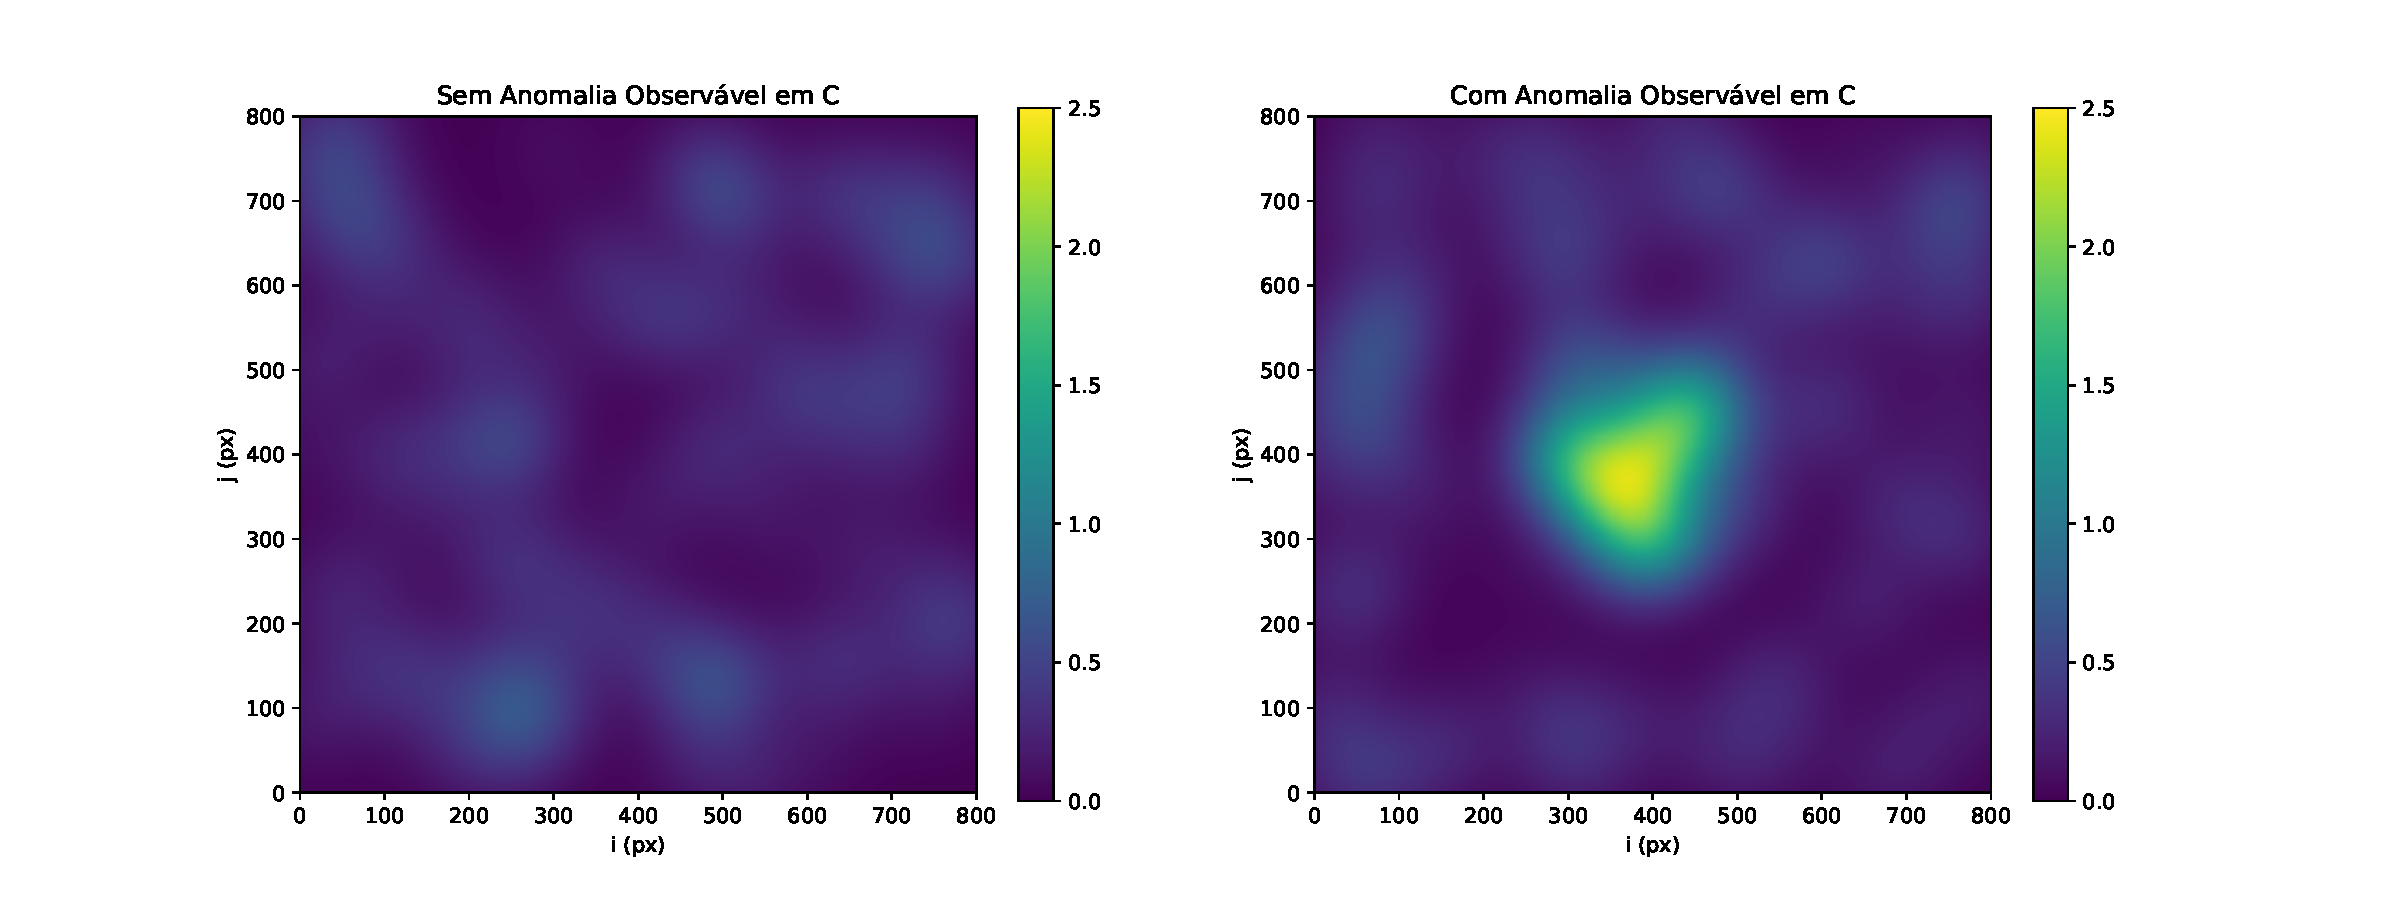
\includegraphics[width=1\linewidth]{./Figures/GaussMap.pdf}
	\label{fig:GaussMap}
\end{figure}

Sabendo que as operações definidas em $\mathcal{L}_{\text{total}}$ {\lq\lq}ensinam{\rq\rq} o comportamento aqui postulado e generalizado na Equação \ref{eq:Z(x,y)}, pode-se simular duas situações que esperadas, respectivamente, casos onde não existam anomalias e infortunados casos onde elas estejam presentes. Essa situação está retratada na Figura \ref{fig:GaussMap}, onde uma superfície quase-planar, regida por pequenas oscilações esperadas, é oriunda de uma amostragem ordinária, obtida sobre um operador ou identidade. Simultaneamente, observa-se o caso anômalo, detectado pelo pico proeminente, que quebra a expectativa do encontro de um campo de variações aleatórias isotrópicas.  

Dada uma imagem de secção de MRI, em uma posição qualquer, sempre haverão uma ou duas imagens vizinhas, ao longo da dimensão de empilhamento. Logo observando um objeto de estudo completo, com todas as suas \textit{layers}, uma dinâmica pode ser observada nas flutuações do {\lq\lq}plano{\rq\rq} que constitui o espaço de resoluções. A movimentação esperada no caso não anômalo, deve ser facilmente modulada pelo de ruído Perlin \cite{Perlin1985}, enquanto anomalias devem criar instâncias emergentes.

Se for tomado o comportamento das forças tensoriais dessa malha em função de uma pequena área uniforme, também será visto um comportamento que pode ser descrito e modulado como não tendencioso. Uma maneira de presenciar essa característica seria a verificação da Lei de Benford \cite{Berger2015} sobre os múltiplos aspectos dos dígitos de controle abstraídos dessas unidades tensoriais e suas vizinhanças. Para o caso não anômalo, a tensão efetiva deve ser pouco apreciável, tanto globalmente, quanto localmente. Este comportamento deve ser verdadeiro para ambos os casos, estático e dinâmico.  

O estudo da versão recíproca desse espaço não pode ser negligenciado \cite{Mizrahi2002}, pois a existência de qualquer tipo ou grau de ordem, será, por definição, um forte indicativo da presença de anomalias no objeto de estudo, sejam elas localizadas ou difusas. Em adendo, é preciso reafirmar também que a elaboração e modulação da amplitude $A_{ij}$, torna essa representação espacial condizente entre os $n$ operadores propostos, admitindo a comparação direta e superposição. Com isso, denomina-se a representação espacial proposta como {\lq\lq}Espaço de Resoluções Condizentes{\rq\rq}.


$\frac{}{}$\\
\begin{Large}
	\textbf{3.5 Estrutura de Dados.}
\end{Large}
$\frac{}{}$\\

Como já foi denotada a intenção pelo uso do formato de treinamento não supervisionado\cite{Garg2016,Zhang2022,Nakao2021,Cao2022} e também já estruturada uma metodologia de uso desse treinamento com redes convolucionais, pode-se discutir a forma de aquisição e implementação da base de dados que será utilizada para treinamento. 

Uma vez que o foco está situado em casos elusivos, não aparentes ou virtualmente não observáveis, o uso de dados públicos de bancos de imagem \cite{LaMontagne2019,Marcus2010,Marcus2007,2020, 2025}, pode {\lq\lq}envenenar{\rq\rq} os modelos e inviabilizar o treinamento, visto que se busca estudar algo que justamente não foi devidamente classificado, não se pode cometer o erro de {\lq\lq}inundar{\rq\rq} o modelo com casos que aparentem normalidade, mas já contenham anomalias detectáveis. É claro que isso deve ser lidado naturalmente pelo treinamento não rotulado, mas a possibilidade do normal ser mascarado se não houver cuidados com a disposição da amostragem existe.

Com isso, talvez a segmentação etária e o uso de dados de acompanhamento médico
sejam os candidatos ideais para o presente estudo. Se forem utilizadas estruturas saudáveis de indivíduos relativamente jovens\footnote{Que possuam a estabilização morfológica ordinária esperada pela evolução natural da estrutura que compõe o objeto de estudo.}, onde existe certa segurança na expectativa do comportamento ordinário, um viés problemático pode ser evitado.

Outro ponto curioso é a maneira natural na qual a proposta de elaboração de um espaço de relações condizentes se entrosa com a segregação etária dos dados de treinamento. Se o espaço de relações condizentes for modulado com base em coletas amostrais de indivíduos relativamente jovens e supondo que a evolução natural da morfologia atue uniformemente sobre o objeto de estudo, o efeito etário deve atuar sobre o \textit{ground state} do espaço. Talvez flutuações de maior magnitude apareçam, contudo, sua modulação será esperada e seguramente terão ordens de grandeza de diferença em relação às anomalias detectáveis.

Outra possibilidade interessante, mas computacionalmente custosa, seria o treinamento pareado de múltiplos modelos para múltiplas faixas etárias utilizando técnicas de \textit{transfer learning} e \textit{ensemble learning} \cite{Xue2020}. Seria possível congelar essas redes já treinadas e repetir o procedimento de convolução \cite{Jha2024, Iman2023}, para isso seria tomada uma camada de entrada composta por \textit{stacks} de CNNs, que passaria por um \textit{Pooling}, depois Convolução, \textit{Pooling}, \textit{Flattening \& Bottleneck} e, por fim, os \textit{heads} de saída. Efetivamente essa abordagem tem potencial para conciliar todos os operadores propostos e diferentes faixas etárias por meio de um modelo hierárquico, onde o procedimento acima descrito é repetido para o treinamento de uma CNN para o conjunto de operadores e o processo é repetido para segmentação etária\footnote{Dentro da gama de expectativa de normalidade.}. 

Vale ressaltar que a estipulação de um modelo hierárquico gera uma rede, cujo tempo de execução é substancialmente maior do que uma CNN comum, contudo o custo de hardware de treinamento também é expressivamente inferior do que seria requerido para uma rede com tamanha entrada. Na próxima seção, será discutido como as estruturas convolucionais podem ser representadas por algoritmos de computação quântica.

$\frac{}{}$\\
\begin{Large}
	\textbf{3.6 Redes Neurais Convolucionais Quânticas.}
\end{Large}
$\frac{}{}$\\


Além da CNN clássica, o presente projeto busca explorar o potencial da computação quântica na construção de redes neurais convolucionais híbridas, onde os algoritmos quânticos serão utilizados como filtros não-lineares a fim de enriquecer a extração de características antes da etapa de classificação convencional em uma CNN clássica \cite{Garg2020}. O objetivo principal é empregar transformações unitárias no espaço de Hilbert para identificar padrões e realçar características sutis nas imagens de ressonância magnética, buscando facilitar a detecção de anomalias pouco evidentes. O processamento quântico é incorporado como uma etapa inicial na \textit{pipeline} da CNN \cite{Oh}, onde os dados são codificados em estados quânticos, manipulados por portas quânticas que funcionam como filtros convolucionais e, por fim, medidos para gerar representações otimizadas que alimentam a CNN clássica.

Inicialmente, a imagem de entrada passa por uma etapa de pré-processamento, onde suas informações serão codificadas em um estado quântico. Esta codificação pode ser feita utilizando técnicas como \textit{Amplitude Encoding}, que permite representar a intensidade dos pixels na amplitude de um vetor de estado, ou \textit{Angle Encoding}, que associa as intensidades a rotações de qubits em torno de eixos específicos na esfera de Bloch \cite{Divya}. Essa transformação permite que toda a imagem seja processada em paralelo, aproveitando o paralelismo inerente da computação quântica. Além disso, essa representação codificada garante que informações espaciais da imagem sejam preservadas, facilitando a construção de filtros quânticos especializados.

Uma vez que os dados estão representados em um estado quântico, serão utilizadas operações unitárias para aplicar filtros convolucionais \cite{Chen2022}. Essas operações são escolhidas para realizar transformações específicas sobre o estado, destacando padrões de interesse que podem estar ocultos na imagem original. No contexto deste projeto, serão explorados os circuitos variacionais parametrizados, onde os parâmetros dos filtros são ajustáveis e treináveis. Esses filtros quânticos podem atuar de forma semelhante às convoluções em redes neurais clássicas, mas com a vantagem de explorar transformações no espaço de Hilbert, onde correlações não triviais entre diferentes regiões da imagem podem emergir devido ao emaranhamento entre os qubits. A ideia é buscar detectar variações morfológicas que, de outra forma, poderiam ser negligenciadas por filtros clássicos tradicionais.

Após a aplicação dos filtros quânticos, o próximo passo envolve a extração da informação processada por meio de medições nos qubits. Como a computação quântica é intrinsecamente probabilística, diferentes estratégias de medição são consideradas para garantir que as informações mais relevantes sejam extraídas. Por exemplo, pode-se realizar medições em uma base computacional para obter histogramas de distribuição das características extraídas ou medições em bases alternativas que fornecem informações sobre a estrutura de correlações não triviais entre diferentes partes da imagem. O resultado dessas medições gera um conjunto de \textit{features} transformadas, que serão posteriormente inseridas na CNN clássica para as etapas finais de classificação e segmentação.

A combinação entre os filtros quânticos e a CNN clássica cria um pipeline híbrido \cite{Divya, Chen2022} que tem o potencial de melhorar a eficiência da rede neural sem aumentar significativamente sua complexidade computacional. Enquanto a CNN tradicional aprende padrões a partir de convoluções com kernels clássicos, o módulo quântico fornece filtros adicionais que ampliam a capacidade do modelo de capturar estruturas sutis. Essa abordagem híbrida tem o potencial de reduzir a necessidade de dados rotulados, pois os filtros quânticos podem destacar variações morfológicas complexas sem depender exclusivamente do treinamento supervisionado. Além disso, a metodologia proposta é escalável e pode ser aplicada a diferentes modalidades de imagem, oferecendo uma solução versátil para problemas de diagnóstico médico.

$\frac{}{}$\\
\begin{Large}
	\textbf{3.7 Projetores Identitários}
\end{Large}
$\frac{}{}$\\

O formalismo dos projetores de Mori \cite{Mori1965} foi desenvolvido originalmente para que sistemas com diferentes componentes possam ser separados com base na natureza dessas componentes. Um exemplo disso é a separação de sistemas dinâmicos em suas componentes lentas e rápidas. Neste projeto, pretende-se instrumentalizar a formulação geral dos projetores para caracterizar diferentes tipos de perfis recorrentes ou coincidentes obtidos como resultado da aplicação do treinamento há pouco elaborado.

Imagine que é obtido um conjunto de perfis radiais associados ($| \mathbf{a}_{\theta} \rangle$) a uma patologia qualquer, ou a uma anomalia coesa. É possível testar como esse perfil se correlaciona com outro perfil qualquer, em outras palavras, pode-se verificar quais partes de $| \mathbf{a}_{\theta} \rangle$ estão contidas no subespaço dos perfis radiais $| \mathbf{v}_{\theta} \rangle$, com isso o projetor ($\mathcal{P}$) captura apenas as partes do perfil testado que estão alinhadas ao alvo. Tomando a matriz de correlação ($\text{C}_{\theta,\theta'}$) como exemplo, a seguinte equação pode ser escrita:
\begin{align}
	\mathcal{P} | \mathbf{a}_{\theta} \rangle = \sum_{\theta,\theta'}^{M} \langle \mathbf{a}_{\theta} | \mathbf{v}_\theta \rangle \, (C^{-1})_{\theta,\theta'} \, | \mathbf{v}_{\theta'} \rangle.
	\label{eq:Mori}
\end{align}

Essa abordagem parece, a primeira vista, pouco factível, mas é preciso lembrar que foi proposta uma metodologia capaz de recriar a matriz de correlação angular com base nos modos dominantes, o que gera um {\lq\lq}sinal{\rq\rq} limpo, portanto testável. Logo, pode-se facilmente descobrir o operador que deu origem a perturbação espacial que evidenciou a anomalia. Desse modo, todo arcabouço ferramental para a utilização de projetores como elementos classificadores de anomalias já está contido no presente projeto. 

A adição desse formalismo ao projeto agrega a ele a capacidade de criar máscaras não truncadas, ou seja, relacionadas a própria estrutura morfológica cerebral, automaticamente adaptáveis e transponíveis. Efetivamente, esses projetores permitem não apenas a classificação, mas sim a superposição das componentes extraídas da imagem original. Um ponto curioso é que essa dinâmica de projetores e máscaras é um sub-produto da metodologia de aquisição e treinamento apresentada. 

$\frac{}{}$\\
\hrule $\frac{}{}$\\
\begin{LARGE}
	\textbf{4. Cronograma}
\end{LARGE}
\\ \hrule $\frac{}{}$\par

A execução do presente projeto está proposta para 36 meses, nos quais o seguinte cronograma é sugerido:
\begin{itemize}
    \item Durante o primeiro ano, o protótipo, já funcional, aqui apresentado será transposto para sua versão operacional. Será feita uma revisão da bibliografia em prol da acomodação das perspectivas atuais ao foco das futuras publicações. Serão selecionados os primeiros operadores como método de aquisição e terá início o treinamento das redes.
    \item No segundo ano, a abordagem inicial será extrapolada para outras elaborações sobre o espaço vetorial, como a correlação angular, densidade angular e busca por possíveis malhas semi-regulares alvejáveis por intermédio dos operadores angulares.
    \item O terceiro ano focará na aplicação dos conceitos propostos e estudados nos anos anteriores em Redes Neurais Convolucionais Quânticas.
\end{itemize}

Todas as etapas contarão com publicações em revistas de impacto apreciável e devidamente indexadas. Serão tabuladas e disponibilizadas, como biblioteca aberta, todas as ferramentas e modelos aqui desenvolvidos.

\newpage
%$\frac{}{}$\\
\hrule $\frac{}{}$\\
\begin{LARGE}
	\textbf{5. Disseminação}
\end{LARGE}
\\ \hrule $\frac{}{}$\par
\label{chap:disseminacao}

A prerrogativa central é a produção de uma metodologia que permita o estudo e a redução da dimensionalidade de imagens MRI, idealmente desenvolvida para treinamento de redes neurais adversas. Contudo, vale frisar que a abordagem proposta para descobertas de anomalias em imagens pode apresentar-se aplicável a outras semânticas, principalmente aquelas versadas sobre influência de diretrizes radiais, como radares ópticos com lentes parabólicas.   

Logo no primeiro ano, a presente proposta deve se elencar como alternativa viável em relação a técnicas consagradas de uso geral. Deve ocorrer também a liberação da primeira versão estável da biblioteca de operadores, cujos resultados foram enunciados nesse projeto como {\lq\lq}construtos virtuais{\rq\rq}\footnote{Projeções abstratas da realidade que revelam informações obscuras.}, utilizados na etapa de aquisição e estudo dos dados. Notavelmente, essa abordagem vem concatenada à sua publicação.

O estudo da correlação angular provavelmente transporá mais de um ano,  no entanto, é de se esperar que seus primeiros resultados já sejam publicados ao longo do primeiro ano, em conjunção com outros operadores mais triviais. Devido ao escopo sucinto deste projeto, não foi possível abordar outros operadores, similares a correlação angular, que já apresentaram resultados proeminentes durante a prototipagem, como densidade angular e entropia. Esses e outros também serão investigados ao longo do primeiro ano.

Do segundo ano em diante, serão abordadas as prerrogativas mais elaboradas, como o estudo de aplicações concatenadas de operadores, assim como o estudo da instrumentalização da superposição dos resultados obtidos no espaço proposto como objeto de treinamento de novas redes neurais, possivelmente mais acuradas do que as anteriores. 

Desse ponto em diante, é esperado o tratamento da transposição do que já foi estudado para as aplicações nas Redes Neurais Convolucionais Quânticas, contudo há de se supor que esse será o tema dominante da pesquisa no terceiro ano. 

Por fim, o terceiro ano será especialmente destinado a publicações e conferencias. Em completude, partes não exploradas desse projeto devem ser utilizadas para constituição de projetos de pesquisa relacionados.

\bibliographystyle{ieeetr}
\bibliography{bibliografia-pos-doc}		
\end{document} 
